\mfpicnumber{1}

\opengraphsfile{TrigEquIneq}

\setcounter{footnote}{0}

\label{TrigEquIneq}

In Sections \ref{TheUnitCircle}, \ref{CircularFunctions} and most recently \ref{ArcTrig}, we solved some basic equations involving the trigonometric functions. Below we summarize the techniques we've employed thus far.  Note that we use the neutral letter `$u$' as the argument\footnote{See the comments at the beginning of Section \ref{TrigGraphs} for a review of this concept.} of each circular function for generality.

\smallskip

\phantomsection
\label{trigeqnstrategy1}

\colorbox{ResultColor}{\bbm
\centerline{\textbf{Strategies for Solving Basic Equations Involving Trigonometric Functions}}

\smallskip

\begin{itemize}

\item To solve $\cos(u) = c$ or $\sin(u) = c$ for $-1 \leq c \leq 1$, first solve for $u$ in the interval $[0,2\pi)$ and add integer multiples of the period $2\pi$.  If $c < -1$ or of $c > 1$, there are no real solutions.

\item To solve $\sec(u) = c$ or $\csc(u) = c$ for $c \leq -1$ or $c \geq 1$,  convert to cosine or sine, respectively, and solve as above.  If $-1 < c < 1$, there are no real solutions.

\item To solve  $\tan(u) = c$ for any real number $c$,  first solve for $u$ in the interval $\left(-\frac{\pi}{2}, \frac{\pi}{2}\right)$ and add integer multiples of the period $\pi$.

\item  To solve  $\cot(u) = c$ for $c \neq 0$, convert to tangent and solve as above.  If $c = 0$, the solution to $\cot(u) = 0$ is $u = \frac{\pi}{2} + \pi k$ for integers $k$.

\end{itemize}

\ebm}

\smallskip

Using the above guidelines, we can comfortably solve $\sin(x) = \frac{1}{2}$ and find the solution $x = \frac{\pi}{6} + 2\pi k$ or $x = \frac{5\pi}{6} + 2\pi k$ for integers $k$. How do we solve something like $\sin(3x) = \frac{1}{2}$?  Since this equation has the \textit{form} $\sin(u) = \frac{1}{2}$, we know the solutions take the form  $u= \frac{\pi}{6} + 2\pi k$ or $u = \frac{5\pi}{6} + 2\pi k$ for integers $k$. Since the argument of sine here is $3x$, we have $3x= \frac{\pi}{6} + 2\pi k$ or $3x = \frac{5\pi}{6} + 2\pi k$ for integers $k$. To solve for $x$, we divide both sides\footnote{Don't forget to divide the $2\pi k$ by $3$ as well!} of these equations by $3$, and obtain $x = \frac{\pi}{18} + \frac{2\pi}{3} k$ or $x = \frac{5\pi}{18} + \frac{2\pi}{3}k$ for integers $k$.  This is the technique employed in the example below.

\begin{ex}  \label{TrigEqnEx1} Solve the following equations and check your answers analytically.  List the solutions which lie in the interval $[0,2\pi)$ and verify them using a graphing utility.


\begin{multicols}{3}

\begin{enumerate}

\item  $\cos(2x) = -\frac{\sqrt{3}}{2}$
\item  $\csc\left(\frac{1}{3}x-\pi \right) = \sqrt{2}$
\item  $\cot\left(3x \right) = 0$

\setcounter{HW}{\value{enumi}}

\end{enumerate}

\end{multicols}

\begin{multicols}{3} 

\begin{enumerate}

\setcounter{enumi}{\value{HW}}

\item  $\sec^{2}(x) = 4$
\item  \label{arctanin02pi} $\tan\left(\frac{x}{2}\right) = -3$
\item  $\sin(2x) = 0.87$

\end{enumerate}

\end{multicols}

{\bf Solution.}

\begin{enumerate}

\item  The solutions to $\cos(u) =-\frac{\sqrt{3}}{2}$ are $u = \frac{5\pi}{6} + 2\pi k$ or $u = \frac{7\pi}{6} + 2\pi k$ for integers $k$.  Since the argument of cosine here is $2x$, this means $2x = \frac{5\pi}{6} + 2\pi k$ or $2x = \frac{7\pi}{6} + 2\pi k$ for integers $k$.  Solving for $x$ gives $x = \frac{5\pi}{12} + \pi k$ or $x = \frac{7\pi}{12} + \pi k$ for integers $k$.  To check these answers analytically, we substitute them into the original equation.  For any integer $k$ we have

\[ \begin{array}{rclr}

\cos\left( 2\left[\frac{5\pi}{12} + \pi k\right]\right) &  = &  \cos\left(\frac{5\pi}{6} + 2\pi k\right) & \\ [3pt]
																												& =  &   \cos\left(\frac{5\pi}{6}\right) & \text{(the period of cosine is $2\pi$)} \\ [3pt]
																												& =  & -\frac{\sqrt{3}}{2} & \\
\end{array}\] 

Similarly, we find $\cos\left( 2\left[\frac{7\pi}{12} + \pi k\right]\right) = \cos\left(\frac{7\pi}{6} + 2\pi k\right) = \cos\left(\frac{7\pi}{6}\right) = -\frac{\sqrt{3}}{2}$.  To determine which of our solutions lie in $[0,2\pi)$, we substitute integer values for $k$.  The solutions we keep come from the values of $k = 0$ and $k =1$ and are  $x = \frac{5\pi}{12}$,  $\frac{7\pi}{12}$, $\frac{17\pi}{12}$ and $\frac{19\pi}{12}$.  Using a calculator, we graph $y = \cos(2x)$ and $y = -\frac{\sqrt{3}}{2}$ over $[0,2\pi)$ and examine where these two graphs intersect.  We see that the $x$-coordinates of the intersection points correspond to the decimal representations of our exact answers.

\item  Since this equation has the form $\csc(u) = \sqrt{2}$, we rewrite this as $\sin(u) = \frac{\sqrt{2}}{2}$ and find $u = \frac{\pi}{4} + 2\pi k$ or $u = \frac{3\pi}{4} + 2\pi  k$ for integers $k$.  Since the argument of cosecant here is $\left(\frac{1}{3}x-\pi \right)$,

\[ \frac{1}{3}x-\pi = \frac{\pi}{4} + 2\pi k \quad \text{or} \quad  \frac{1}{3}x-\pi = \frac{3\pi}{4} + 2\pi k\]


To solve $\frac{1}{3}x-\pi = \frac{\pi}{4} + 2\pi k$, we first add $\pi$ to both sides

\[ \frac{1}{3} x = \frac{\pi}{4} + 2\pi k + \pi\]

A common error is to treat the `$2\pi k$' and `$\pi$' terms as `like' terms and try to combine them when they are not.\footnote{Do you see why?}  We can, however, combine the `$\pi$' and `$\frac{\pi}{4}$' terms to get

\[ \frac{1}{3} x = \frac{5\pi}{4} + 2\pi k\]

We now finish by multiplying both sides by $3$ to get

\[ x = 3 \left( \frac{5\pi}{4} + 2\pi k \right) = \frac{15 \pi}{4} + 6\pi k \]

Solving the other equation, $\frac{1}{3}x-\pi = \frac{3\pi}{4} + 2\pi k$ produces $x = \frac{21\pi}{4} + 6 \pi k$ for integers $k$. To check the first family of answers, we substitute, combine line terms, and simplify.

\[ \begin{array}{rclr}

\csc\left(\frac{1}{3} \left[ \frac{15\pi}{4} + 6 \pi  k \right] - \pi   \right)  &  = &  \csc\left(\frac{5\pi}{4} + 2\pi k - \pi \right) & \\ [3pt]
																												& =  &   \csc\left(\frac{\pi}{4} + 2\pi k\right) &  \\ [3pt]
																												& =  & \csc\left(\frac{\pi}{4}\right) & \text{(the period of cosecant is $2\pi$)} \\
																												& = & \sqrt{2} & \\
\end{array}\] 



The family $x= \frac{21\pi}{4} + 6 \pi  k$ checks similarly.  Despite having infinitely many solutions, we find that \textit{none} of them lie in $[0,2\pi)$.  To verify this graphically, we use a reciprocal identity to rewrite the cosecant as a sine and we find that $y = \frac{1}{\sin\left(\frac{1}{3}x-\pi\right)}$ and $y =\sqrt{2}$ do not intersect at all over the interval $[0,2\pi)$.


\begin{center}

\begin{tabular}{cc}

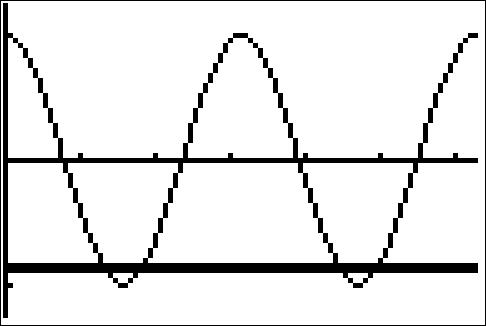
\includegraphics[width=2in]{./IntroTrigGraphics/TrigEquIneq01.jpg} &

\hspace{0.75in} 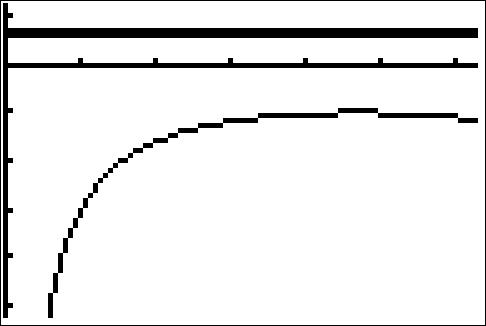
\includegraphics[width=2in]{./IntroTrigGraphics/TrigEquIneq02.jpg} \\

 $y = \cos(2x)$ and  \boldmath $y=-\frac{\sqrt{3}}{2}$ & 

 \hspace{0.75in}  $y = \frac{1}{\sin\left(\frac{1}{3}x-\pi\right)}$ and \boldmath $y =\sqrt{2}$ \\
 
\end{tabular}

\end{center}

\item  Since $\cot(3x) = 0$ has the form $\cot(u) = 0$, we know $u = \frac{\pi}{2} + \pi k$, so, in this case,  $3x =  \frac{\pi}{2} + \pi k$ for integers $k$.  Solving for $x$ yields $x = \frac{\pi}{6} + \frac{\pi}{3} k$.  Checking our answers, we get

\[ \begin{array}{rclr}

\cot\left(3\left[ \frac{\pi}{6} + \frac{\pi}{3} k\right]\right)  &  = &  \cot\left(\frac{\pi}{2} + \pi k\right)  & \\ [3pt]
																												& =  &   \cot\left(\frac{\pi}{2}\right) &  \text{(the period of cotangent is $\pi$)} \\ [3pt]
																												& =  & 0 & \\
																								
\end{array}\] 



 As $k$ runs through the integers, we obtain six answers, corresponding to $k=0$ through $k=5$, which lie in $[0, 2\pi)$: $x = \frac{\pi}{6}$, $\frac{\pi}{2}$, $\frac{5\pi}{6}$, $\frac{7\pi}{6}$ , $\frac{3\pi}{2}$ and  $\frac{11\pi}{6}$. To confirm these graphically, we must be careful. On many calculators, there is no function button for cotangent.  We choose\footnote{The reader is encouraged to see what happens if we had chosen the reciprocal identity $\cot(3x) = \frac{1}{\tan(3x)}$ instead.  The graph on the calculator \textit{appears} identical, but what happens when you try to find the intersection points?} to use the quotient identity  $\cot(3x) = \frac{\cos(3x)}{\sin(3x)}$.  Graphing $y = \frac{\cos(3x)}{\sin(3x)}$ and $y = 0$ (the $x$-axis), we see that the $x$-coordinates of the intersection points approximately match our solutions.

\item The complication in solving an equation like $\sec^{2}(x) = 4$ comes not from the argument of secant, which is just $x$, but rather, the fact the secant is being squared.  To get this equation to look like one of the forms listed on page \pageref{trigeqnstrategy1}, we extract square roots to get $\sec(x) = \pm 2$. Converting to cosines, we have  $\cos(x) = \pm \frac{1}{2}$.  For $\cos(x) = \frac{1}{2}$, we get $x = \frac{\pi}{3} + 2\pi k$ or $x = \frac{5\pi}{3} + 2\pi k$ for integers $k$.  For $\cos(x) = -\frac{1}{2}$, we get $x = \frac{2\pi}{3} + 2\pi k$ or $x = \frac{4\pi}{3} + 2\pi k$ for integers $k$.  If we take a step back and think of these families of solutions geometrically, we see we are finding the measures of all angles with a reference angle of $\frac{\pi}{3}$.  As a result, these solutions can be combined and we may write our solutions as $x = \frac{\pi}{3} + \pi k$ and $x = \frac{2\pi}{3} + \pi k$ for integers $k$.  To check the first family of solutions, we note that, depending on the integer $k$,  $\sec\left(\frac{\pi}{3} + \pi k\right)$ doesn't always equal $\sec\left(\frac{\pi}{3}\right)$.  However, it is true that for all integers $k$,  $\sec\left(\frac{\pi}{3} + \pi k\right) = \pm \sec\left(\frac{\pi}{3}\right) = \pm 2$.  (Can you show this?)  As a result, 


\[ \begin{array}{rclr}

\sec^{2}\left(\frac{\pi}{3} + \pi k\right)  &  = &  \left( \pm \sec\left(\frac{\pi}{3}\right)\right)^2  & \\ [3pt]
																												& =  &   (\pm 2)^2 &  \\ [3pt]
																												& =  & 4 & \\
																								
\end{array}\] 

The same holds for the family $x =\frac{2\pi}{3} + \pi k$.  The solutions which lie in $[0,2\pi)$ come from the values $k = 0$ and $k=1$, namely $x = \frac{\pi}{3}$, $\frac{2\pi}{3}$, $\frac{4\pi}{3}$ and $\frac{5\pi}{3}$.  To confirm graphically, we use a reciprocal identity to rewrite the secant as cosine.  The $x$-coordinates of the intersection points of  $y = \frac{1}{(\cos(x))^2}$ and $y = 4$ verify our answers.


\begin{center}

\begin{tabular}{cc}

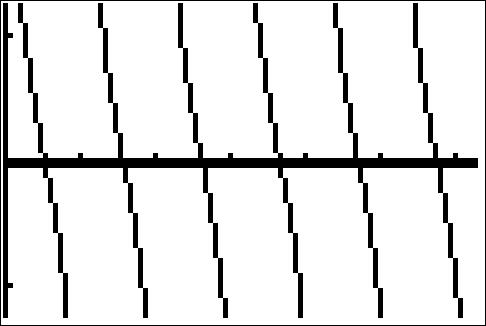
\includegraphics[width=2in]{./IntroTrigGraphics/TrigEquIneq03.jpg} &

\hspace{0.75in} 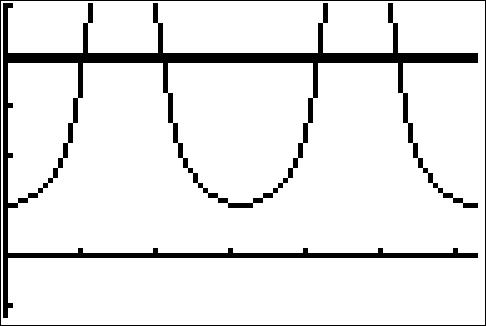
\includegraphics[width=2in]{./IntroTrigGraphics/TrigEquIneq04.jpg} \\

  $y = \frac{\cos(3x)}{\sin(3x)}$ and \boldmath $y=0$   & 

 \hspace{0.75in}   $y = \frac{1}{\cos^{2}(x)}$ and \boldmath $y = 4$  \\

\end{tabular}

\end{center}

\item  The equation  $\tan\left(\frac{x}{2}\right) = -3$ has the form $\tan(u) = -3$, whose solution is $u = \arctan(-3) + \pi k$.  Hence, $\frac{x}{2} = \arctan(-3) + \pi k$, so  $x = 2\arctan(-3) + 2\pi k$ for integers $k$.  To check, we note

\[ \begin{array}{rclr}

\tan\left(\frac{2\arctan(-3) + 2\pi k}{2}\right)  &  = & \tan\left( \arctan(-3) + \pi k \right)  & \\ [3pt]
																												& =  & \tan\left(\arctan(-3) \right) & \text{(the period of tangent is $\pi$)} \\ [3pt]
																												& =  & -3 & (\text{See Theorem } \ref{arctangentcotangentfunctionprops}) \\
																								
\end{array}\] 


 To determine which of our answers lie in the interval $[0,2\pi)$, we first need to get an idea of the value of $2\arctan(-3)$.  While we could easily find an approximation using a calculator,\footnote{Your instructor will let you know if you should abandon the analytic route at this point and use your calculator.  But seriously, what fun would that be?} we proceed analytically.  Since $-3 < 0$, it follows that $-\frac{\pi}{2} < \arctan(-3) < 0$.  Multiplying through by $2$ gives $-\pi < 2\arctan(-3) < 0$.   We are now in a position to argue which of the solutions $x = 2\arctan(-3) + 2\pi k$ lie in $[0,2\pi)$.  For $k = 0$, we get $x = 2\arctan(-3) < 0$, so we discard this answer and all answers $x = 2\arctan(-3) + 2\pi k$ where $k < 0$.  Next, we turn our attention to $k = 1$ and get $x = 2\arctan(-3) + 2\pi$. Starting with the inequality $-\pi < 2\arctan(-3) < 0$, we add $2\pi$  and get $\pi < 2\arctan(-3) +2\pi < 2\pi$.  This means $x = 2\arctan(-3) + 2\pi$ lies in $[0,2\pi)$.  Advancing $k$ to $2$ produces $x = 2\arctan(-3) + 4\pi$. Once again, we get from $-\pi < 2\arctan(-3) < 0$ that $3\pi < 2\arctan(-3) + 4\pi < 4\pi$.  Since this is outside the interval $[0,2\pi)$,  we discard $x = 2\arctan(-3) + 4\pi$ and all solutions of the form $x = 2\arctan(-3) + 2\pi k$ for $k > 2$.   Graphically, we see $y = \tan\left(\frac{x}{2}\right)$ and $y = -3$ intersect only once on $[0,2\pi)$ at $x = 2\arctan(-3) + 2\pi\approx 3.7851$.

\item To solve $\sin(2x) = 0.87$, we first note that it has the form $\sin(u) = 0.87$, which has the family of solutions $u = \arcsin(0.87) + 2\pi k$ or $u =\pi -  \arcsin(0.87) + 2\pi k$ for integers $k$. Since the argument of sine here is $2x$, we get $2x = \arcsin(0.87) + 2\pi k$ or $2x =\pi -  \arcsin(0.87) + 2\pi k$ which gives $x = \frac{1}{2} \arcsin(0.87) + \pi k$ or $x =\frac{\pi}{2} -  \frac{1}{2}\arcsin(0.87) + \pi k$ for integers $k$.  To check,

\[ \begin{array}{rclr}

\sin\left(2\left[\frac{1}{2} \arcsin(0.87) + \pi k\right]\right)  &  = & \sin\left(\arcsin(0.87) + 2\pi k\right)  & \\ [3pt]
																													& =  & \sin\left(\arcsin(0.87)\right) & \text{(the period of sine is $2\pi$)} \\ [3pt]
																												& =  & 0.87& (\text{See Theorem } \ref{arccosinesinefunctionprops})\\
																								
\end{array}\] 


For the family $x =\frac{\pi}{2} -  \frac{1}{2}\arcsin(0.87) + \pi k$ , we get

\[ \begin{array}{rclr}

\sin\left(2\left[\frac{\pi}{2} - \frac{1}{2} \arcsin(0.87) + \pi k\right]\right)  &  = & \sin\left(\pi - \arcsin(0.87) + 2\pi k\right) & \\ [3pt]
																												& =  & \sin\left(\pi - \arcsin(0.87)\right) & \text{(the period of sine is $2\pi$)} \\ [3pt]
																												& =  & \sin\left(\arcsin(0.87)\right) & \text{($\sin(\pi - t) = \sin(t)$)} \\ [3pt]
																												& =  & 0.87& (\text{See Theorem } \ref{arccosinesinefunctionprops}) \\
																								
\end{array}\] 

To determine which of these solutions lie in $[0,2\pi)$, we first need to get an idea of the value of $x=\frac{1}{2} \arcsin(0.87)$.  Once again, we could use the calculator, but we adopt an analytic route here.  By definition, $0 < \arcsin(0.87) < \frac{\pi}{2}$ so that multiplying through by $\frac{1}{2}$ gives us $0 < \frac{1}{2} \arcsin(0.87) < \frac{\pi}{4}$.  Starting with the family of solutions $x = \frac{1}{2} \arcsin(0.87) + \pi k$, we use the same kind of arguments as in our solution to number \ref{arctanin02pi} above and find only the solutions corresponding to $k =0$ and $k=1$ lie in $[0,2\pi)$:  $x = \frac{1}{2} \arcsin(0.87)$ and $x = \frac{1}{2} \arcsin(0.87) + \pi$.  Next, we move to the family $x =\frac{\pi}{2} -  \frac{1}{2}\arcsin(0.87) + \pi k$ for integers $k$. Here, we need to get a better estimate of $\frac{\pi}{2} - \frac{1}{2} \arcsin(0.87)$.  From the inequality $0 < \frac{1}{2}\arcsin(0.87) < \frac{\pi}{4}$, we first multiply through by $-1$ and then add $\frac{\pi}{2}$ to get $\frac{\pi}{2} > \frac{\pi}{2} -\frac{1}{2} \arcsin(0.87) >  \frac{\pi}{4}$, or $\frac{\pi}{4} < \frac{\pi}{2} -\frac{1}{2} \arcsin(0.87) < \frac{\pi}{2}$.  Proceeding with the usual arguments, we find the only solutions which lie in $[0,2\pi)$ correspond to $k = 0$ and $k=1$, namely $x =\frac{\pi}{2} -  \frac{1}{2}\arcsin(0.87)$ and  $x = \frac{3\pi}{2} - \frac{1}{2}\arcsin(0.87)$. All told, we have found four solutions to $\sin(2x) = 0.87$ in $[0,2\pi)$:  $x =\frac{1}{2} \arcsin(0.87)$, $x=\frac{1}{2} \arcsin(0.87) + \pi$, $x =\frac{\pi}{2} -  \frac{1}{2}\arcsin(0.87)$ and  $x = \frac{3\pi}{2} - \frac{1}{2}\arcsin(0.87)$. By graphing $y = \sin(2x)$ and $y = 0.87$, we confirm our results.

\enlargethispage*{.5in}

\begin{center}

\begin{tabular}{cc}

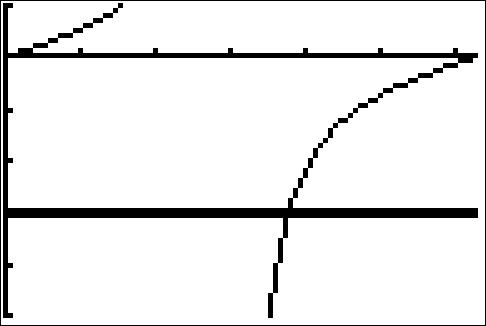
\includegraphics[width=2in]{./IntroTrigGraphics/TrigEquIneq05.jpg} &

\hspace{0.75in} 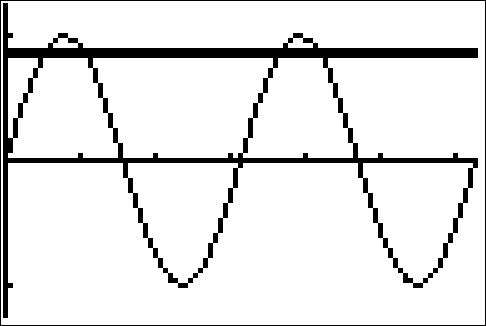
\includegraphics[width=2in]{./IntroTrigGraphics/TrigEquIneq06.jpg} \\

$y = \tan\left(\frac{x}{2}\right)$ and \boldmath $y = -3$    & 

 \hspace{0.75in}  $y = \sin(2x)$ and \boldmath $y = 0.87$ \\

\end{tabular}

\end{center} 

\end{enumerate}

\vspace*{-.3in} \qed

\end{ex}

\pagebreak

Each of the problems in Example \ref{TrigEqnEx1} featured one trigonometric function.  If an equation involves two different trigonometric functions or if the equation contains the same trigonometric function but with different arguments, we will need to use identities and Algebra to reduce the equation to the same form as those given on page  \pageref{trigeqnstrategy1}.
 
\begin{ex} \label{TrigEqIdEx1}  Solve the following equations and list the solutions which lie in the interval $[0,2\pi)$.  Verify your solutions on $[0,2\pi)$ graphically.

\begin{multicols}{2}

\begin{enumerate}

\item  $3\sin^{3}(x) = \sin^{2}(x)$
\item $\sec^{2}(x) = \tan(x) + 3$

\setcounter{HW}{\value{enumi}}

\end{enumerate}

\end{multicols}

\begin{multicols}{2}

\begin{enumerate}

\setcounter{enumi}{\value{HW}}

\item   $\cos(2x) = 3\cos(x) - 2$
\item  $\cos(3x) = 2- \cos(x)$

\setcounter{HW}{\value{enumi}}

\end{enumerate}

\end{multicols}

\begin{multicols}{2}

\begin{enumerate}

\setcounter{enumi}{\value{HW}}

\item  $\cos(3x) = \cos(5x)$
\item $\sin(2x) =\sqrt{3} \cos(x)$

\setcounter{HW}{\value{enumi}}

\end{enumerate}

\end{multicols}

\begin{multicols}{2}

\begin{enumerate}

\setcounter{enumi}{\value{HW}}

\item  $\sin(x)\cos\left(\frac{x}{2}\right) + \cos(x)\sin\left(\frac{x}{2}\right) = 1$
\item  $\cos(x) - \sqrt{3} \sin(x) = 2$

\end{enumerate}
 
\end{multicols}

{\bf Solution.}

\begin{enumerate}

\item We resist the temptation to divide both sides of $3\sin^{3}(x) = \sin^{2}(x)$ by $\sin^{2}(x)$ (What goes wrong if you do?) and instead gather all of the terms to one side of the equation and factor.

\[ \begin{array}{rclr}

3\sin^{3}(x) & = &  \sin^{2}(x) & \\
3\sin^{3}(x) -  \sin^{2}(x) & = & 0 &  \\
\sin^{2}(x) (3 \sin(x) - 1) & = & 0 & \text{Factor out $\sin^{2}(x)$ from both terms.} \\ \end{array} \]

We get $\sin^{2}(x) = 0$ or $3\sin(x) - 1 = 0$. Solving for $\sin(x)$, we find  $\sin(x) = 0$ or $\sin(x) = \frac{1}{3}$.  The solution to the first equation is $x = \pi k$, with $x = 0$ and $x = \pi$ being the two solutions which lie in $[0,2\pi)$.  To solve $\sin(x) = \frac{1}{3}$, we use the arcsine function to get $x = \arcsin\left(\frac{1}{3}\right) + 2\pi k$ or $x = \pi - \arcsin\left(\frac{1}{3}\right) + 2\pi k$ for integers $k$. We find the two solutions here which lie in $[0,2\pi)$ to be $x = \arcsin\left(\frac{1}{3}\right)$ and $x = \pi - \arcsin\left(\frac{1}{3}\right)$.  To check graphically, we plot $y = 3(\sin(x))^3$ and $y = (\sin(x))^2$ and find the  $x$-coordinates of the intersection points of these two curves.  Some extra zooming is required near $x=0$ and $x=\pi$ to verify that these two curves do in fact intersect four times.\footnote{Note that we are \textit{not} counting the point $(2\pi,0)$ in our solution set since $x = 2\pi$ is not in the interval $[0,2\pi)$. In the forthcoming solutions, remember that while  $x = 2\pi$ may be a solution to the equation, it isn't counted among the solutions in $[0,2\pi)$.}

\item  Analysis of  $\sec^{2}(x) = \tan(x) + 3$ reveals two different trigonometric functions, so an identity is in order.  Since $\sec^{2}(x) = 1 + \tan^{2}(x)$, we get

\[ \begin{array}{rclr}

\sec^{2}(x) &  = & \tan(x) + 3 & \\
1 + \tan^{2}(x) & = & \tan(x) + 3& \text{(Since $\sec^{2}(x) = 1 + \tan^{2}(x)$.)} \\
\tan^{2}(x) - \tan(x) -2 & = & 0 & \\
u^2 - u - 2 & = & 0 & \text{Let $u = \tan(x)$.} \\
(u + 1)(u - 2) & = & 0 & \\ \end{array} \]

This gives $u = -1$ or $u = 2$.  Since $u = \tan(x)$, we have $\tan(x) = -1$ or $\tan(x) = 2$. From $\tan(x) = -1$, we get $x = -\frac{\pi}{4} + \pi k$ for integers $k$.  To solve $\tan(x) = 2$, we employ the arctangent function and get $x = \arctan(2) + \pi k$ for integers $k$.  From the first set of solutions, we get $x = \frac{3\pi}{4}$ and $x = \frac{5\pi}{4}$ as our answers which lie in $[0,2\pi)$.  Using the same sort of argument we saw in Example \ref{TrigEqnEx1},   we get  $x=\arctan(2)$ and $x = \pi + \arctan(2)$ as answers from our second set of solutions which lie in $[0,2\pi)$.  Using a reciprocal identity, we rewrite the secant as a cosine and graph  $y = \frac{1}{(\cos(x))^2}$ and $y = \tan(x) + 3$ to find the $x$-values of the points where they intersect.


\begin{center}

\begin{tabular}{cc}

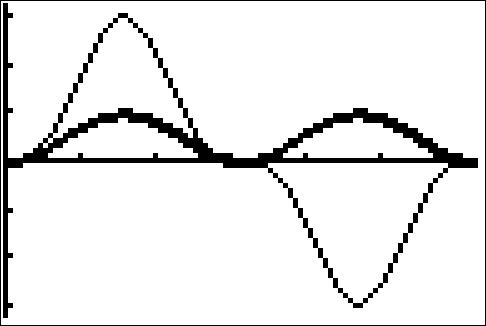
\includegraphics[width=2in]{./IntroTrigGraphics/TrigEquIneq07.jpg} &

\hspace{0.75in} 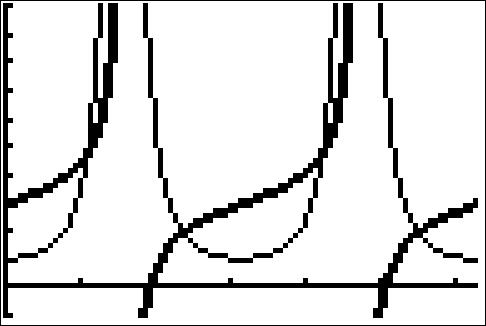
\includegraphics[width=2in]{./IntroTrigGraphics/TrigEquIneq08.jpg} \\

$y = 3(\sin(x))^3$ and \boldmath  $y = (\sin(x))^2$   & 

 \hspace{0.75in} $y = \frac{1}{(\cos(x))^2}$ and \boldmath  $y = \tan(x) + 3$  \\
 
 \end{tabular}

\end{center}

\item  In the equation $\cos(2x) = 3\cos(x) - 2$, we have the same circular function, namely cosine, on both sides but the arguments differ.  Using the identity $\cos(2x) = 2\cos^{2}(x) - 1$, we obtain a `quadratic in disguise' and proceed as we have done in the past.

\[ \begin{array}{rclr}

\cos(2x) & = & 3\cos(x) - 2 & \\
2\cos^{2}(x) -1 & = & 3\cos(x) -2 & \text{(Since $\cos(2x) = 2\cos^{2}(x) -1$.)} \\
2\cos^{2}(x) - 3\cos(x) +1 & = & 0 & \\
2 u^2 - 3 u + 1 & = & 0 & \text{Let $u = \cos(x)$.}\\
(2u - 1)(u - 1) & = & 0 & \\ \end{array} \]

This gives $u = \frac{1}{2}$ or $u = 1$.  Since $u = \cos(x)$, we get $\cos(x) = \frac{1}{2}$ or $\cos(x) = 1$.  Solving  $\cos(x) = \frac{1}{2}$, we get $x = \frac{\pi}{3} + 2\pi k$ or $x = \frac{5\pi}{3} + 2\pi k$ for integers $k$.  From $\cos(x) = 1$, we get $x = 2\pi k$ for integers $k$.  The answers which lie in $[0,2\pi)$ are $x =0$,  $\frac{\pi}{3}$, and $\frac{5\pi}{3}$.  Graphing $y = \cos(2x)$ and $y = 3\cos(x) - 2$, we find, after a little extra effort, that the curves intersect in three places on $[0,2\pi)$, and  the $x$-coordinates of these points confirm our results.


\item  To solve $\cos(3x) = 2- \cos(x)$, we use the same technique as in the previous problem.  From Example \ref{doubleangleex}, number \ref{cosinepolynomial}, we know that $\cos(3x) = 4\cos^{3}(x) - 3\cos(x)$.  This transforms the equation into a polynomial in terms of $\cos(x)$.


\[ \begin{array}{rclr}

\cos(3x) & = &2- \cos(x) & \\
4\cos^{3}(x) - 3\cos(x) & = & 2- \cos(x) & \\
2\cos^{3}(x) - 2\cos(x) -2  & = & 0 & \\
4 u^3 - 2 u -2  & = & 0 & \text{Let $u = \cos(x)$.} \\ \end{array} \]

To solve $4u^3-2u-2=0$, we need the techniques in Chapter \ref{Polynomials} to factor $4u^3-2u-2$ into $(u-1)\left(4u^2+4u+2\right)$.  We get either $u-1 = 0$ or  $4u^2+2u+2=0$, and since the discriminant of the latter is negative, the only real solution to $4u^3-2u-2=0$ is $u = 1$.  Since $u = \cos(x)$, we get $\cos(x) = 1$, so $x = 2\pi k$ for integers $k$.  The only solution which lies in $[0,2\pi)$ is $x = 0$.  Graphing $y = \cos(3x)$ and $y = 2- \cos(x)$ on the same set of axes over $[0,2\pi)$ shows that the graphs intersect at what appears to be $(0,1)$, as required.

\begin{center}

\begin{tabular}{cc}

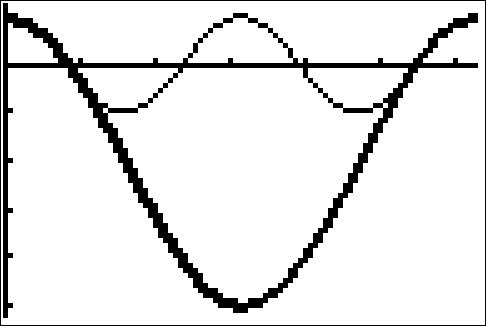
\includegraphics[width=2in]{./IntroTrigGraphics/TrigEquIneq09.jpg} &

\hspace{0.75in} 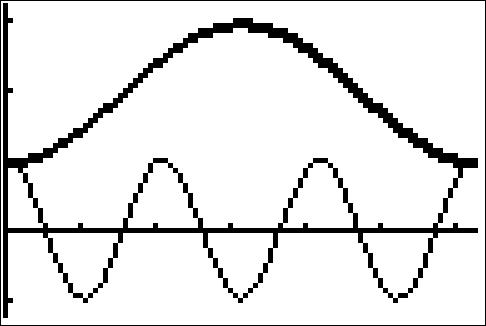
\includegraphics[width=2in]{./IntroTrigGraphics/TrigEquIneq10.jpg} \\

$y = \cos(2x)$ and \boldmath  $y = 3\cos(x) - 2$   & 

 \hspace{0.75in} $y = \cos(3x)$ and \boldmath $y = 2- \cos(x)$ \\
 
 \end{tabular}

\end{center}


\item  While we could approach  $\cos(3x) = \cos(5x)$ in the same manner as we did the previous two problems, we choose instead to showcase the utility of the Sum to Product Identities.  From $\cos(3x) = \cos(5x)$, we get $\cos(5x) - \cos(3x) = 0$, and it is the presence of $0$ on the right hand side that indicates a switch to a product would be a good move.\footnote{As always, experience is the greatest teacher here!}  Using Theorem \ref{sumtoproduct}, we have that $\cos(5x) - \cos(3x)  = - 2 \sin\left( \frac{5x + 3x}{2}\right)\sin\left( \frac{5x - 3x}{2}\right) = -2 \sin(4x)\sin(x)$.  Hence, the equation $\cos(5x) = \cos(3x)$ is equivalent to $-2 \sin(4x) \sin(x) = 0$.  From this, we get $\sin(4x) = 0$ or $\sin(x)$ = 0.  Solving $\sin(4x) = 0$ gives $x = \frac{\pi}{4} k$ for integers $k$, and the solution to $\sin(x) = 0$ is $x = \pi k$ for integers $k$.  The second set of solutions is contained in the first set of solutions,\footnote{As always, when in doubt, write it out!} so our final solution to $\cos(5x) = \cos(3x)$ is $x = \frac{\pi}{4} k$ for integers $k$.  There are eight of these answers which lie in $[0,2\pi)$:  $x = 0$, $\frac{\pi}{4}$, $\frac{\pi}{2}$, $\frac{3\pi}{4}$, $\pi$, $\frac{5\pi}{4}$, $\frac{3\pi}{2}$ and $\frac{7\pi}{4}$.  Our plot of the graphs of $y = \cos(3x)$ and $y = \cos(5x)$ below (after some careful zooming) bears this out. 

\item  In examining the equation   $\sin(2x) =\sqrt{3} \cos(x)$, not only do we have different circular functions involved, namely sine and cosine, we also have different arguments to contend with, namely $2x$ and $x$.  Using the identity $\sin(2x) = 2 \sin(x) \cos(x)$ makes all of the arguments the same and we proceed as we would solving any nonlinear equation -- gather all of the nonzero terms on one side of the equation and factor.

\[ \begin{array}{rclr}

\sin(2x) & = & \sqrt{3} \cos(x) & \\
2 \sin(x) \cos(x) & = & \sqrt{3} \cos(x)  & \text{(Since $\sin(2x) = 2\sin(x) \cos(x)$.)} \\
2\sin(x) \cos(x) - \sqrt{3} \cos(x) & = & 0 & \\
\cos(x) (2 \sin(x) - \sqrt{3}) & = & 0 & \\ \end{array} \]

from which we get $\cos(x) = 0$ or $\sin(x) = \frac{\sqrt{3}}{2}$. From $\cos(x) = 0$, we obtain $x = \frac{\pi}{2} + \pi k$ for integers $k$. From $\sin(x) = \frac{\sqrt{3}}{2}$, we get $x = \frac{\pi}{3} + 2\pi k$ or $x = \frac{2\pi}{3} + 2\pi k$ for integers $k$.  The answers which lie in $[0,2\pi)$ are $x = \frac{\pi}{2}$, $\frac{3\pi}{2}$, $\frac{\pi}{3}$ and $\frac{2\pi}{3}$.  We graph $y = \sin(2x)$ and $y = \sqrt{3} \cos(x)$ and, after some careful zooming,  verify our answers.

\begin{center}

\begin{tabular}{cc}

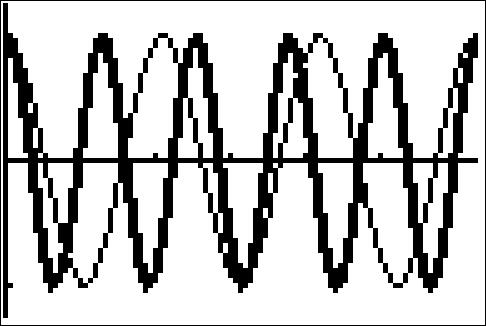
\includegraphics[width=2in]{./IntroTrigGraphics/TrigEquIneq11.jpg} &

\hspace{0.75in} 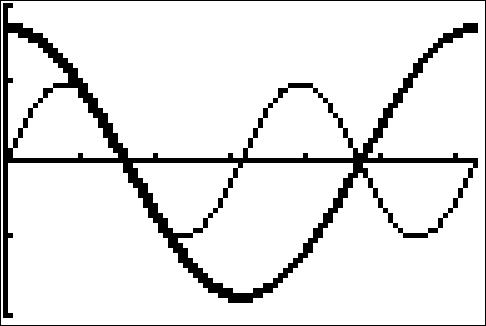
\includegraphics[width=2in]{./IntroTrigGraphics/TrigEquIneq12.jpg} \\

$y = \cos(3x)$ and \boldmath $y = \cos(5x)$    & 

 \hspace{0.75in} $y = \sin(2x)$ and \boldmath $y = \sqrt{3} \cos(x)$  \\
 
 \end{tabular}

\end{center}

\item Unlike the previous problem, there seems to be no quick way to get the circular functions or their arguments to match in the equation $\sin(x)\cos\left(\frac{x}{2}\right) + \cos(x)\sin\left(\frac{x}{2}\right) = 1$.  If we stare at it long enough, however,  we realize that the left hand side is the expanded form of the sum formula for $\sin\left(x + \frac{x}{2}\right)$.  Hence, our original equation is equivalent to  $\sin\left(\frac{3}{2} x\right) = 1$.  Solving, we find $x = \frac{\pi}{3} + \frac{4\pi}{3} k$ for integers $k$.  Two of these solutions lie in $[0,2\pi)$: $x = \frac{\pi}{3}$ and $x = \frac{5\pi}{3}$. Graphing $y = \sin(x)\cos\left(\frac{x}{2}\right) + \cos(x)\sin\left(\frac{x}{2}\right)$ and $y = 1$ validates our solutions.

\item  With the absence of double angles or squares, there doesn't seem to be much we can do.  However, since the arguments of the cosine and sine are the same, we can rewrite the left hand side of this equation as a sinusoid.\footnote{We are essentially `undoing' the sum / difference formula for cosine or sine, depending on which form we use, so this problem is actually closely related to the previous one!}  To fit $f(x) = \cos(x) - \sqrt{3} \sin(x)$ to the form $A\sin(\omega t + \phi) + B$, we use what we learned in Example \ref{expandedsinusoidex1} and find $A = 2$, $B = 0$, $\omega = 1$ and $\phi = \frac{5\pi}{6}$.   Hence, we can rewrite the equation  $\cos(x) - \sqrt{3} \sin(x) = 2$  as $2 \sin\left(x + \frac{5\pi}{6}\right) = 2$, or $\sin\left(x + \frac{5\pi}{6}\right) = 1$.  Solving the latter, we get $x  = - \frac{\pi}{3} + 2\pi k$ for integers $k$. Only one of these solutions, $x = \frac{5\pi}{3}$, which corresponds to $k=1$, lies in $[0,2\pi)$.  Geometrically, we see that $y = \cos(x) - \sqrt{3} \sin(x)$ and $y = 2$ intersect just once, supporting our answer.

\begin{center}

\begin{tabular}{cc}

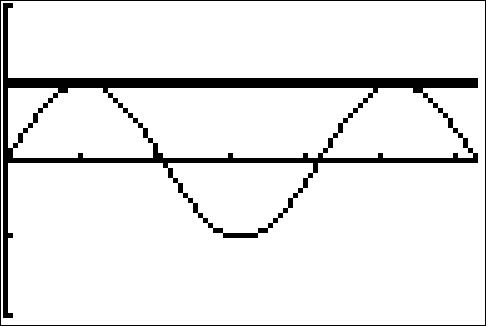
\includegraphics[width=2in]{./IntroTrigGraphics/TrigEquIneq13.jpg} &

\hspace{0.25in} 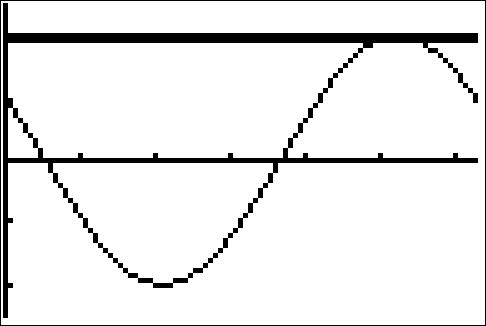
\includegraphics[width=2in]{./IntroTrigGraphics/TrigEquIneq14.jpg} \\

$y = \sin(x)\cos\left(\frac{x}{2}\right) + \cos(x)\sin\left(\frac{x}{2}\right)$ and \boldmath $y = 1$     & 

 \hspace{0.25in}  $y = \cos(x) - \sqrt{3} \sin(x)$ and \boldmath $y = 2$ \\

\end{tabular}

\end{center}

\end{enumerate}
\vspace{-.25in} \qed
\end{ex}
 
We repeat here the advice given when solving systems of nonlinear equations in section \ref{NonLinear} --  when it comes to solving equations involving the trigonometric functions, it helps to just try something.  

Next, we focus on solving inequalities involving the trigonometric functions.  Since these functions are continuous on their domains, we may use the sign diagram technique we've used in the past to solve the inequalities.\footnote{See page \pageref{firstsigndiagram}, Example \ref{polygraphex}, page \pageref{rationalsigndiagram}, page \pageref{algebraicsigndiagram}, Example \ref{expineq} and Example \ref{logineq} for discussion of this technique.}

\begin{ex}  \label{TrigIneqEx1} Solve the following inequalities on $[0,2\pi)$.  Express your answers using interval notation and verify your answers graphically.

\begin{multicols}{3}

\begin{enumerate}

\item  $2\sin(x) \leq 1$

\item  $\sin(2x) > \cos(x)$

\item  $\tan(x) \geq 3$

\end{enumerate}

\end{multicols}

{\bf Solution.}

\begin{enumerate}

\item  We begin solving $2\sin(x) \leq 1$ by collecting all of the terms on one side of the equation and zero on the other to get $2\sin(x) - 1 \leq 0$.  Next, we let $f(x) = 2\sin(x) - 1$ and note that our original inequality is equivalent to solving $f(x) \leq 0$. We now look to see where, if ever, $f$ is undefined and where $f(x) = 0$.  Since the domain of $f$ is all real numbers, we can immediately set  about finding the zeros of $f$.  Solving $f(x) = 0$, we have $2\sin(x) - 1=0$ or $\sin(x) = \frac{1}{2}$.  The solutions here are $x = \frac{\pi}{6} + 2\pi k$ and $x = \frac{5\pi}{6} + 2\pi k$ for integers $k$.  Since we are restricting our attention to $[0,2\pi)$, only $x = \frac{\pi}{6}$ and $x = \frac{5\pi}{6}$ are of concern to us.  Next, we choose test values in $[0,2\pi)$ other than the zeros and determine if $f$ is positive or negative there.  For $x = 0$ we have $f(0) = -1$, for $x = \frac{\pi}{2}$ we get $f\left(\frac{\pi}{2}\right) = 1$ and for $x = \pi$ we get $f(\pi) = -1$.  Since our original inequality is equivalent to $f(x) \leq 0$, we are looking for where the function is negative $(-)$ or $0$, and we get the intervals $\left[0, \frac{\pi}{6}\right] \cup \left[\frac{5\pi}{6}, 2\pi \right)$.  We can confirm our answer graphically by seeing where the graph of $y = 2\sin(x)$ crosses or is below the graph of $y = 1$. 

\begin{center}

\begin{tabular}{m{2in}c}

\begin{mfpic}[10]{-6}{6}{-2}{2}
\polyline{(-6,0),(6,0)}
\xmarks{-6,-2,2,6}
\tiny
\tlpointsep{6pt}
\normalsize
\tlabel[cc](-6,-1){$0$}
\tlabel[cc](-4,1){$(-)$}
\tlabel[cc](-2,-1){$\frac{\pi}{6}$}
\tlabel[cc](-2,1){0}
\tlabel[cc](0,1){$(+)$}
\tlabel[cc](2,-1){$\frac{5\pi}{6}$}
\tlabel[cc](2,1){$0$}
\tlabel[cc](4,1){$(-)$}
\tlabel[cc](6,-1){$2\pi$}
\end{mfpic} 

& 

\hspace{.75in} 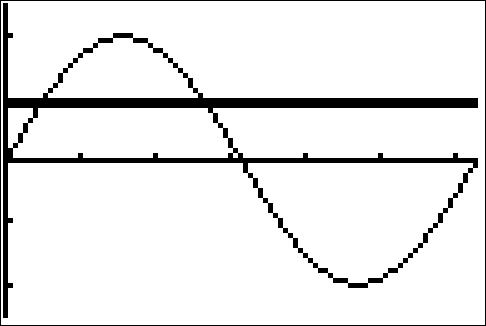
\includegraphics[width=2in]{./IntroTrigGraphics/TrigEquIneq15.jpg} \\

& \hspace{.75in} $y = 2\sin(x)$ and \boldmath $y = 1$ \\

\end{tabular}

\end{center}


\item  We first rewrite  $\sin(2x) > \cos(x)$   as $\sin(2x) - \cos(x) > 0$ and let $f(x) = \sin(2x) - \cos(x)$.  Our original inequality is thus equivalent to $f(x) > 0$. The domain of $f$ is all real numbers, so we can advance to finding the zeros of $f$.  Setting $f(x) = 0$ yields $\sin(2x) - \cos(x) = 0$, which, by way of the double angle identity for sine, becomes $2\sin(x)\cos(x) - \cos(x) = 0$ or $\cos(x) (2\sin(x) - 1) = 0$.  From $\cos(x) = 0$, we get $x = \frac{\pi}{2} + \pi k$ for integers $k$ of which only $x = \frac{\pi}{2}$ and $x = \frac{3\pi}{2}$ lie in $[0,2\pi)$.  For $2\sin(x) - 1 = 0$, we get $\sin(x) = \frac{1}{2}$ which gives $x = \frac{\pi}{6} + 2\pi k$ or $x = \frac{5\pi}{6} + 2\pi k$ for integers $k$.  Of those, only $x = \frac{\pi}{6}$ and $x = \frac{5\pi}{6}$ lie in $[0,2\pi)$.  Next, we choose our test values.  For $x =0$ we find $f(0) = -1$; when $x = \frac{\pi}{4}$ we get $f\left(\frac{\pi}{4}\right) =1 - \frac{\sqrt{2}}{2} = \frac{2 - \sqrt{2}}{2}$;  for $x = \frac{3\pi}{4}$ we get $f\left(\frac{3\pi}{4}\right) =-1 + \frac{\sqrt{2}}{2} =  \frac{\sqrt{2} - 2}{2}$;  when $x=\pi$ we have $f(\pi) = 1$, and lastly, for $x = \frac{7\pi}{4}$ we get $f\left(\frac{7\pi}{4}\right) = -1 - \frac{\sqrt{2}}{2} =  \frac{-2 - \sqrt{2}}{2}$.  We see $f(x) > 0$ on $\left(\frac{\pi}{6}, \frac{\pi}{2}\right) \cup \left(\frac{5\pi}{6}, \frac{3\pi}{2}\right)$, so this is our answer.  We can use the calculator to check that the graph of $y = \sin(2x)$ is indeed above the graph of $y = \cos(x)$ on those intervals. 

\begin{center}
\begin{tabular}{m{2in}c}

\begin{mfpic}[10]{-10}{10}{-2}{2}
\polyline{(-10,0),(10,0)}
\xmarks{-10,-6,-2,2,6,10}
\tiny
\tlpointsep{6pt}
\normalsize
\tlabel[cc](-10,-1){$0$}
\tlabel[cc](-8,1){$(-)$}
\tlabel[cc](-6,-1){$\frac{\pi}{6}$}
\tlabel[cc](-6,1){0}
\tlabel[cc](-4,1){$(+)$}
\tlabel[cc](-2,-1){$\frac{\pi}{2}$}
\tlabel[cc](-2,1){0}
\tlabel[cc](0,1){$(-)$}
\tlabel[cc](2,-1){$\frac{5\pi}{6}$}
\tlabel[cc](2,1){0}
\tlabel[cc](4,1){$(+)$}
\tlabel[cc](6,-1){$\frac{3\pi}{2}$}
\tlabel[cc](6,1){0}
\tlabel[cc](8,1){$(-)$}
\tlabel[cc](10,-1){$2\pi$}
\end{mfpic} 

& 

\hspace{1.25in} 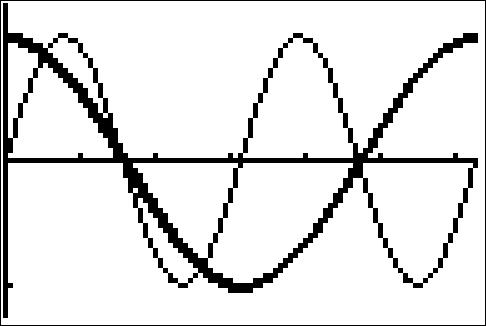
\includegraphics[width=2in]{./IntroTrigGraphics/TrigEquIneq16.jpg} \\

& \hspace{1.25in} $y = \sin(2x)$ and \boldmath $y = \cos(x)$ \\

\end{tabular}

\end{center}

\item  Proceeding as in the last two problems, we rewrite  $\tan(x) \geq 3$ as $\tan(x) - 3 \geq 0$ and let $f(x) = \tan(x) - 3$.  We note that on $[0,2\pi)$, $f$ is undefined at $x =\frac{\pi}{2}$ and $\frac{3\pi}{2}$, so those values will need the usual disclaimer on the sign diagram.\footnote{See page \pageref{rationalsigndiagram} for a discussion of the non-standard character known as the interrobang.}  Moving along to zeros, solving $f(x) = \tan(x) - 3 = 0$ requires the arctangent function.  We find $x = \arctan(3) + \pi k$ for integers $k$ and of these, only $x = \arctan(3)$ and $x = \arctan(3) + \pi$ lie in $[0,2\pi)$.  Since $3 > 0$, we know $0 < \arctan(3) < \frac{\pi}{2}$ which allows us to position these zeros correctly on the sign diagram. To choose test values, we begin with $x=0$ and find $f(0) = -3$. Finding a convenient test value in the interval $\left(\arctan(3), \frac{\pi}{2}\right)$ is a bit more challenging.  Keep in mind that the arctangent function is increasing and is bounded above by $\frac{\pi}{2}$.  This means that the number $x = \arctan(117)$ is guaranteed\footnote{We could have chosen any value $\arctan(t)$ where $t > 3$.} to lie between  $\arctan(3)$ and $\frac{\pi}{2}$.  We see that $f(\arctan(117)) = \tan(\arctan(117)) - 3 = 114$.  For our next test value, we take $x = \pi$ and find $f(\pi) = -3$.  To find our next test value, we note that since $\arctan(3) < \arctan(117) < \frac{\pi}{2}$,  it follows\footnote{\ldots by adding $\pi$ through the inequality \ldots} that $\arctan(3) + \pi < \arctan(117) + \pi < \frac{3\pi}{2}$.  Evaluating $f$ at $x = \arctan(117) + \pi$ yields $f(\arctan(117)+\pi) = \tan(\arctan(117) + \pi) -3 = \tan(\arctan(117)) - 3 = 114$.  We choose our last test value to be $x = \frac{7\pi}{4}$ and find $f\left(\frac{7\pi}{4}\right) = -4$.  Since we want $f(x) \geq 0$, we see that our answer is $\left[ \arctan(3), \frac{\pi}{2}\right) \cup  \left[\arctan(3)+\pi, \frac{3\pi}{2}\right)$.  Using the graphs of $y = \tan(x)$ and $y = 3$, we see when the graph of the former is above (or meets) the graph of the latter.

\begin{center}
\begin{tabular}{m{2in}c}

\begin{mfpic}[10]{-10}{10}{-2}{2}
\polyline{(-10,0),(10,0)}
\xmarks{-10,-6,-2,2,6,10}
\tiny
\tlpointsep{6pt}
\normalsize
\tlabel[cc](-10,-1){$0$}
\tlabel[cc](-8,1){$(-)$}
\tlabel[cc](-6,-1){\tiny $\arctan(3)$}
\tlabel[cc](-6,1){0}
\tlabel[cc](-4,1){$(+)$}
\tlabel[cc](-2,-1){$\frac{\pi}{2}$}
\tlabel[cc](-2,1){\textinterrobang}
\tlabel[cc](0,1){$(-)$}
\tlabel[cc](2,-1){\tiny $(\arctan(3)+\pi)$}
\tlabel[cc](2,1){0}
\tlabel[cc](4,1){$(+)$}
\tlabel[cc](6,-1){$\frac{3\pi}{2}$}
\tlabel[cc](6,1){\textinterrobang}
\tlabel[cc](8,1){$(-)$}
\tlabel[cc](10,-1){$2\pi$}
\end{mfpic} 

& 

\hspace{1.25in} 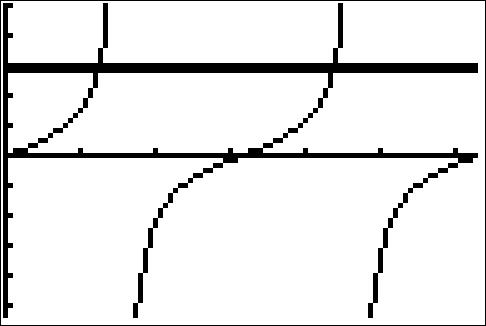
\includegraphics[width=2in]{./IntroTrigGraphics/TrigEquIneq17.jpg} \\

& \hspace{1.25in} $y = \tan(x)$ and \boldmath $y =3$ \\

\end{tabular}

\end{center}


\vspace{-.25in} \qed


\end{enumerate}



\end{ex}


We close this section with an example that puts solving equations and inequalities to good use -- finding domains of functions.


\begin{ex}  \label{TrigDomainEx1} Express the domain of the following functions using extended interval notation.\footnote{See page \pageref{extendedinterval} for details about this notation.}

\begin{multicols}{3}

\begin{enumerate}

\item  $f(x) = \csc\left(2x + \frac{\pi}{3}\right)$

\item  $f(x) = \dfrac{\sin(x)}{2\cos(x) - 1}$

\item  $f(x) = \sqrt{1 - \cot(x)}$

\end{enumerate}

\end{multicols}

{\bf Solution.}

\begin{enumerate}

\item  To find the domain of $f(x) = \csc\left(2x + \frac{\pi}{3}\right)$, we rewrite $f$ in terms of sine as $f(x) = \frac{1}{\sin\left(2x + \frac{\pi}{3}\right)}$.  Since the sine function is defined everywhere, our only concern comes from zeros in the denominator.  Solving $\sin\left(2x + \frac{\pi}{3}\right) = 0$, we get $x = -\frac{\pi}{6} + \frac{\pi}{2} k$ for integers $k$.  In set-builder notation, our domain is  $\left\{ x : x \neq  -\frac{\pi}{6} + \frac{\pi}{2} k \, \text{for integers $k$} \right\}$.  To help visualize the domain,  we follow the old mantra `When in doubt, write it out!' We get $\left\{ x : x \neq  -\frac{\pi}{6}, \frac{2\pi}{6}, -\frac{4\pi}{6}, \frac{5\pi}{6}, -\frac{7\pi}{6}, \frac{8\pi}{6}, \ldots \right\}$, where we have kept the denominators $6$ throughout to help see the pattern.  Graphing the situation on a numberline, we have

\begin{center}

\begin{mfpic}[15]{-6}{6}{-1}{2}
\arrow \reverse \arrow \polyline{(-6,0), (6,0)}
\xmarks{-5,-3,-1,1,3,5}
\tlpointsep{5pt}
\axislabels {x}{{\small $-\frac{7\pi}{6} \hspace{7pt}$} -5,{\small $-\frac{4\pi}{6} \hspace{7pt}$} -3, {\small $-\frac{\pi}{6} \hspace{7pt}$} -1,{\small $\frac{2\pi}{6}$} 1,{\small $\frac{5\pi}{6}$} 3,  {\small $\frac{8\pi}{6}$} 5}

\penwd{1.5}
\arrow \reverse \arrow \polyline{(-5.75,1), (5.75,1)}

\penwd{0.75}

\gclear \circle{(-5,1),0.15}
\circle{(-5,1),0.15}

\gclear \circle{(-3,1),0.15}
\circle{(-3,1),0.15}

\gclear \circle{(-1,1),0.15}
\circle{(-1,1),0.15}

\gclear \circle{(5,1),0.15}
\circle{(5,1),0.15}

\gclear \circle{(3,1),0.15}
\circle{(3,1),0.15}

\gclear \circle{(1,1),0.15}
\circle{(1,1),0.15}

\end{mfpic}

\end{center}

Proceeding as we did on page \pageref{extendedinterval} in Section \ref{circularfunctionsbeyond}, we let $x_{\mbox{\tiny $k$}}$ denote the $k$th number excluded from the domain and we have  $x_{\mbox{\tiny $k$}} = -\frac{\pi}{6} + \frac{\pi}{2} k = \frac{(3k-1)\pi}{6}$ for integers $k$.  The intervals which comprise the domain are of the form $\left(x_{\mbox{\tiny $k$}}, x_{\mbox{\tiny $k+1$}}  \right) = \left(\frac{(3k-1)\pi}{6}, \frac{(3k+2)\pi}{6} \right)$ as $k$ runs through the integers.  Using extended interval notation, we have that the domain is

\[ \bigcup_{k = -\infty}^{\infty}  \left(\dfrac{(3k-1)\pi}{6}, \dfrac{(3k+2)\pi}{6} \right)\]

We can check our answer by substituting in values of $k$ to see that it matches our diagram.


\item  Since the domains of $\sin(x)$ and $\cos(x)$ are all real numbers, the only concern when finding the domain of  $f(x) =  \frac{\sin(x)}{2\cos(x) - 1}$ is division by zero so we set the denominator equal to zero and solve. From $2\cos(x) - 1 = 0$ we get $\cos(x) = \frac{1}{2}$ so that $x = \frac{\pi}{3} + 2\pi k$ or $x = \frac{5\pi}{3} + 2\pi k$ for integers $k$.  Using set-builder notation, the domain is $\left\{ x : x \neq \frac{\pi}{3} + 2\pi k \, \text{and} \, x \neq \frac{5\pi}{3} + 2\pi k \, \text{for integers $k$} \right\}$, or  $\left\{ x : x \neq \pm \frac{\pi}{3}, \pm \frac{5\pi}{3}, \pm \frac{7\pi}{3}, \pm \frac{11\pi}{3}, \ldots \right\}$, so we have

\begin{center}

\begin{mfpic}[15]{-6}{6}{-1}{2}
\arrow \reverse \arrow \polyline{(-8,0), (8,0)}
\xmarks{-7,-5,-3,-1,1,3,5,7}
\tlpointsep{5pt}
\axislabels {x}{{\small $-\frac{11\pi}{3} \hspace{7pt}$} -7,{\small $-\frac{7\pi}{3} \hspace{7pt}$} -5,{\small $-\frac{5\pi}{3} \hspace{7pt}$} -3, {\small $-\frac{\pi}{3} \hspace{7pt}$} -1,{\small $\frac{\pi}{3}$} 1,{\small $\frac{5\pi}{3}$} 3,  {\small $\frac{7\pi}{3}$} 5,  {\small $\frac{11\pi}{3}$} 7}

\penwd{1.5}
\arrow \reverse \arrow \polyline{(-7.75,1), (7.75,1)}

\penwd{0.75}

\gclear \circle{(-7,1),0.15}
\circle{(-7,1),0.15}

\gclear \circle{(-5,1),0.15}
\circle{(-5,1),0.15}

\gclear \circle{(-3,1),0.15}
\circle{(-3,1),0.15}

\gclear \circle{(-1,1),0.15}
\circle{(-1,1),0.15}

\gclear \circle{(7,1),0.15}
\circle{(7,1),0.15}

\gclear \circle{(5,1),0.15}
\circle{(5,1),0.15}

\gclear \circle{(3,1),0.15}
\circle{(3,1),0.15}

\gclear \circle{(1,1),0.15}
\circle{(1,1),0.15}


\end{mfpic}

\end{center}

Unlike the previous example, we have \textit{two} different families of points to consider, and we present two ways of dealing with this kind of situation.  One way is to generalize what we did in the previous example and use the formulas we found in our domain work to describe the intervals.  To that end, we let  $a_{\mbox{\tiny $k$}} = \frac{\pi}{3} + 2\pi k = \frac{(6k+1)\pi}{3}$ and  $b_{\mbox{\tiny $k$}} = \frac{5\pi}{3} + 2\pi k = \frac{(6k+5) \pi}{3}$ for integers $k$.  The goal now is to write the domain in terms of the $a$'s an $b$'s.  We find $a_{\mbox{\tiny $0$}} =  \frac{\pi}{3}$, $a_{\mbox{\tiny $1$}} =  \frac{7\pi}{3}$,  $a_{\mbox{\tiny $-1$}} =  -\frac{5\pi}{3}$, $a_{\mbox{\tiny $2$}} =  \frac{13\pi}{3}$, $a_{\mbox{\tiny $-2$}} =  -\frac{11\pi}{3}$, $b_{\mbox{\tiny $0$}} =  \frac{5\pi}{3}$,  $b_{\mbox{\tiny $1$}} =  \frac{11\pi}{3}$, $b_{\mbox{\tiny $-1$}} =  -\frac{\pi}{3}$,  $b_{\mbox{\tiny $2$}} =  \frac{17\pi}{3}$  and $b_{\mbox{\tiny $-2$}} =  -\frac{7\pi}{3}$.  Hence, in terms of the $a$'s and $b$'s, our domain is

\[\ldots  \left(a_{\mbox{\tiny $-2$}}, b_{\mbox{\tiny $-2$}}  \right) \cup \left(b_{\mbox{\tiny $-2$}}, a_{\mbox{\tiny $-1$}}  \right)\cup \left(a_{\mbox{\tiny $-1$}}, b_{\mbox{\tiny $-1$}}  \right)\cup \left(b_{\mbox{\tiny $-1$}}, a_{\mbox{\tiny $0$}}  \right)\cup \left(a_{\mbox{\tiny $0$}}, b_{\mbox{\tiny $0$}}  \right)\cup \left(b_{\mbox{\tiny $0$}}, a_{\mbox{\tiny $1$}}  \right)\cup \left(a_{\mbox{\tiny $1$}}, b_{\mbox{\tiny $1$}}  \right)\cup \dots \]

If we group these intervals in pairs, $ \left(a_{\mbox{\tiny $-2$}}, b_{\mbox{\tiny $-2$}}  \right) \cup \left(b_{\mbox{\tiny $-2$}}, a_{\mbox{\tiny $-1$}}  \right)$, $\left(a_{\mbox{\tiny $-1$}}, b_{\mbox{\tiny $-1$}}  \right)\cup \left(b_{\mbox{\tiny $-1$}}, a_{\mbox{\tiny $0$}}  \right)$, $\left(a_{\mbox{\tiny $0$}}, b_{\mbox{\tiny $0$}}  \right)\cup \left(b_{\mbox{\tiny $0$}}, a_{\mbox{\tiny $1$}}  \right)$ and so forth, we see a pattern emerge of the form  $\left(a_{\mbox{\tiny $k$}}, b_{\mbox{\tiny $k$}}  \right)\cup \left(b_{\mbox{\tiny $k$}}, a_{\mbox{\tiny $k+1$}}  \right)$ for integers $k$ so that our domain can be written as 

\[ \bigcup_{k = -\infty}^{\infty} \left(a_{\mbox{\tiny $k$}}, b_{\mbox{\tiny $k$}}  \right)\cup \left(b_{\mbox{\tiny $k$}}, a_{\mbox{\tiny $k+1$}}  \right) =  \bigcup_{k = -\infty}^{\infty} \left(\frac{(6k+1)\pi}{3}, \frac{(6k+5) \pi}{3}  \right)\cup \left(\frac{(6k+5) \pi}{3}, \frac{(6k+7)\pi}{3}  \right) \]

A second approach to the problem exploits the periodic nature of $f$.  Since $\cos(x)$ and $\sin(x)$ have period $2\pi$, it's not too difficult to show the function $f$ repeats itself every $2\pi$ units.\footnote{This doesn't necessarily mean the period of $f$ is $2\pi$.  The tangent function is comprised of $\cos(x)$ and $\sin(x)$, but its period is half theirs.  The reader is invited to investigate the period of $f$.}  This means if we can find a formula for the domain on an interval of length $2\pi$, we can express the entire domain by translating our answer left and right on the $x$-axis by adding integer multiples of $2\pi$. One such interval that arises from our domain work is  $\left[\frac{\pi}{3}, \frac{7\pi}{3}\right]$. The portion of the domain here is  $\left(\frac{\pi}{3}, \frac{5\pi}{3}\right) \cup \left(\frac{5\pi}{3}, \frac{7\pi}{3}\right)$.  Adding integer multiples of $2\pi$, we get the family of intervals  $\left(\frac{\pi}{3} + 2\pi k, \frac{5\pi}{3} + 2\pi k \right) \cup \left(\frac{5\pi}{3} + 2\pi k, \frac{7\pi}{3} + 2\pi k\right)$ for integers $k$.  We leave it to the reader to show that getting common denominators leads to our previous answer.

\pagebreak

\item  To find the domain of $f(x) = \sqrt{1-\cot(x)}$, we first note that, due to the presence of the $\cot(x)$ term, $x \neq \pi k$ for integers $k$.  Next, we recall that for the square root to be defined, we need $1 - \cot(x) \geq 0$.  Unlike the inequalities we solved in Example \ref{TrigIneqEx1}, we are not restricted here to a given interval.  Our strategy is to solve this inequality over $(0,\pi)$  (the same interval which generates a fundamental cycle of cotangent) and then add integer multiples of the period, in this case, $\pi$.  We let $g(x) = 1 - \cot(x)$ and set about making a sign diagram for $g$ over the interval $(0,\pi)$ to find where $g(x) \geq 0$.  We note that $g$ is undefined for $x = \pi k$ for integers $k$, in particular, at the endpoints of our interval $x = 0$ and $x = \pi$. Next, we look for the zeros of $g$.  Solving $g(x) = 0$, we get $\cot(x) = 1$ or $x = \frac{\pi}{4} + \pi k$ for integers $k$ and only one of these, $x = \frac{\pi}{4}$, lies in $(0,\pi)$.   Choosing the test values $x = \frac{\pi}{6}$ and $x = \frac{\pi}{2}$, we get $g\left(\frac{\pi}{6}\right) = 1 - \sqrt{3}$, and $g\left(\frac{\pi}{2}\right) = 1$.  

\begin{center}
\begin{mfpic}[10]{-2}{6}{-2}{2}
\polyline{(-2,0),(6,0)}
\xmarks{-2,2,6}
\tiny
\tlpointsep{6pt}
\normalsize
\tlabel[cc](-2,-1){$0$}
\tlabel[cc](-2,1){\textinterrobang}
\tlabel[cc](0,1){$(-)$}
\tlabel[cc](2,-1){$\frac{\pi}{4}$}
\tlabel[cc](2,1){$0$}
\tlabel[cc](4,1){$(+)$}
\tlabel[cc](6,-1){$\pi$}
\tlabel[cc](6,1){\textinterrobang}
\end{mfpic} 
\end{center}

We find $g(x) \geq 0$ on $\left[\frac{\pi}{4}, \pi \right)$.  Adding multiples of the period we get our solution to consist of the intervals  $\left[\frac{\pi}{4} + \pi k, \pi + \pi k  \right) = \left[\frac{(4k+1)\pi}{4}, (k+1)\pi \right)$.  Using extended interval notation, we express our final answer as

\[\bigcup_{k = -\infty}^{\infty} \left[\dfrac{(4k+1)\pi}{4}, (k+1)\pi \right)\]



\end{enumerate}
\qed
\end{ex}
 
 
\newpage

\subsection{Exercises}

In Exercises \ref{solvebasicfirst} - \ref{solvebasiclast}, find \underline{all} of the exact solutions of the  equation and then list those solutions which are in the interval $[0, 2\pi)$.

\begin{multicols}{3}

\begin{enumerate}

\item $\sin \left( 5x \right) = 0$ \vphantom{$\dfrac{\sqrt{3}}{2}$} \label{solvebasicfirst}
\item $\cos \left( 3x \right) = \dfrac{1}{2}$ \vphantom{$\dfrac{\sqrt{3}}{2}$}
\item $\sin \left( -2x \right) = \dfrac{\sqrt{3}}{2}$ 

\setcounter{HW}{\value{enumi}}

\end{enumerate}

\end{multicols}

\begin{multicols}{3}

\begin{enumerate}

\setcounter{enumi}{\value{HW}}

\item $\tan \left( 6x \right) = 1$
\item $\csc \left( 4x \right) = -1$
\item $\sec \left( 3x \right) = \sqrt{2}$

\setcounter{HW}{\value{enumi}}

\end{enumerate}

\end{multicols}

\begin{multicols}{3}

\begin{enumerate}

\setcounter{enumi}{\value{HW}}

\item $\cot \left( 2x \right) = -\dfrac{\sqrt{3}}{3}$
\item $\cos \left( 9x \right) = 9$ \vphantom{$\dfrac{\sqrt{3}}{2}$}
\item $\sin \left( \dfrac{x}{3} \right) = \dfrac{\sqrt{2}}{2}$

\setcounter{HW}{\value{enumi}}

\end{enumerate}

\end{multicols}

\begin{multicols}{3}

\begin{enumerate}

\setcounter{enumi}{\value{HW}}

\item $\cos \left( x + \dfrac{5\pi}{6} \right) = 0$
\item $\sin \left( 2x - \dfrac{\pi}{3} \right) = -\dfrac{1}{2}$
\item $2\cos \left( x + \dfrac{7\pi}{4} \right) = \sqrt{3}$

\setcounter{HW}{\value{enumi}}

\end{enumerate}

\end{multicols}

\begin{multicols}{3}

\begin{enumerate}

\setcounter{enumi}{\value{HW}}

\item $\csc(x) = 0$
\item $\tan \left( 2x - \pi \right) = 1$
\item $\tan^{2} \left( x \right) = 3$

\setcounter{HW}{\value{enumi}}

\end{enumerate}

\end{multicols}

\begin{multicols}{3}

\begin{enumerate}

\setcounter{enumi}{\value{HW}}

\item $\sec^{2} \left( x \right) = \dfrac{4}{3}$
\item $\cos^{2} \left( x \right) = \dfrac{1}{2}$
\item $\sin^{2} \left( x \right) = \dfrac{3}{4}$ \label{solvebasiclast}

\setcounter{HW}{\value{enumi}}

\end{enumerate}

\end{multicols}

In Exercises \ref{solveidentfirst} - \ref{solveidentlast}, solve the equation, giving the exact solutions which lie in $[0, 2\pi)$

\begin{multicols}{2}

\begin{enumerate}

\setcounter{enumi}{\value{HW}}

\item $\sin \left( x \right) = \cos \left( x \right)$ \label{solveidentfirst}
\item $\sin \left( 2x \right) = \sin \left( x \right)$

\setcounter{HW}{\value{enumi}}

\end{enumerate}

\end{multicols}

\begin{multicols}{2}

\begin{enumerate}

\setcounter{enumi}{\value{HW}}

\item $\sin \left( 2x \right) = \cos \left( x \right)$
\item $\cos \left( 2x \right) = \sin \left( x \right)$

\setcounter{HW}{\value{enumi}}

\end{enumerate}

\end{multicols}

\begin{multicols}{2}

\begin{enumerate}

\setcounter{enumi}{\value{HW}}

\item $\cos \left( 2x \right) = \cos \left( x \right)$
\item  $\cos(2x) = 2 - 5\cos(x)$

\setcounter{HW}{\value{enumi}}

\end{enumerate}

\end{multicols}

\begin{multicols}{2}

\begin{enumerate}

\setcounter{enumi}{\value{HW}}

\item  $3\cos(2x) + \cos(x) + 2 = 0$
\item  $\cos(2x) = 5\sin(x) - 2$

\setcounter{HW}{\value{enumi}}

\end{enumerate}

\end{multicols}

\begin{multicols}{2}

\begin{enumerate}

\setcounter{enumi}{\value{HW}}

\item  $3\cos(2x) = \sin(x) + 2$
\item  $2\sec^{2}(x) = 3 - \tan(x)$

\setcounter{HW}{\value{enumi}}

\end{enumerate}

\end{multicols}

\begin{multicols}{2}

\begin{enumerate}

\setcounter{enumi}{\value{HW}}

\item  $\tan^{2}(x) = 1-\sec(x)$
\item  $\cot^{2}(x) = 3\csc(x) - 3$

\setcounter{HW}{\value{enumi}}

\end{enumerate}

\end{multicols}

\begin{multicols}{2}

\begin{enumerate}

\setcounter{enumi}{\value{HW}}

\item  $\sec(x) = 2\csc(x)$
\item  $\cos(x)\csc(x)\cot(x) = 6-\cot^{2}(x)$

\setcounter{HW}{\value{enumi}}

\end{enumerate}

\end{multicols}

\begin{multicols}{2}

\begin{enumerate}

\setcounter{enumi}{\value{HW}}

\item  $\sin(2x) = \tan(x)$
\item  $\cot^{4}(x) = 4\csc^{2}(x) - 7$

\setcounter{HW}{\value{enumi}}

\end{enumerate}

\end{multicols}

\begin{multicols}{2}

\begin{enumerate}

\setcounter{enumi}{\value{HW}}

\item  $\cos(2x) + \csc^{2}(x) = 0$
\item $\tan^{3} \left( x \right) = 3\tan \left( x \right)$

\setcounter{HW}{\value{enumi}}

\end{enumerate}

\end{multicols}

\begin{multicols}{2}

\begin{enumerate}

\setcounter{enumi}{\value{HW}}

\item $\tan^{2} \left( x \right) = \dfrac{3}{2} \sec \left( x \right)$
\item $\cos^{3} \left( x \right) = -\cos \left( x \right)$ \vphantom{$\dfrac{3}{2}$}

\setcounter{HW}{\value{enumi}}

\end{enumerate}

\end{multicols}

\begin{multicols}{2}

\begin{enumerate}

\setcounter{enumi}{\value{HW}}

\item $\tan (2x) - 2\cos(x) = 0$
\item $\csc^{3}(x) + \csc^{2}(x) = 4\csc(x) + 4$

\setcounter{HW}{\value{enumi}}

\end{enumerate}

\end{multicols}
\enlargethispage{.5in}
\vspace{-.1in}
\begin{multicols}{2}

\begin{enumerate}

\setcounter{enumi}{\value{HW}}

\item $2\tan(x) = 1 - \tan^{2}(x)$
\item $\tan \left( x \right) = \sec \left( x \right)$ \label{solveidentlast}

\setcounter{HW}{\value{enumi}}

\end{enumerate}

\end{multicols}

In Exercises \ref{solvemoreidentfirst} - \ref{solvemoreidentlast}, solve the equation, giving the exact solutions which lie in $[0, 2\pi)$

\begin{multicols}{2}

\begin{enumerate}

\setcounter{enumi}{\value{HW}}

\item $\sin(6x) \cos(x) = -\cos(6x) \sin(x)$ \label{solvemoreidentfirst}
\item  $\sin(3x)\cos(x) = \cos(3x) \sin(x)$

\setcounter{HW}{\value{enumi}}

\end{enumerate}

\end{multicols}

\begin{multicols}{2}

\begin{enumerate}

\setcounter{enumi}{\value{HW}}

\item $\cos(2x)\cos(x) + \sin(2x)\sin(x) = 1$ \vphantom{$\dfrac{\sqrt{3}}{2}$}
\item \small $\cos(5x)\cos(3x) - \sin(5x)\sin(3x) = \dfrac{\sqrt{3}}{2}$ \normalsize

\setcounter{HW}{\value{enumi}}

\end{enumerate}

\end{multicols}

\begin{multicols}{2}

\begin{enumerate}

\setcounter{enumi}{\value{HW}}

%Sinusoids
\item $\sin(x) + \cos(x) = 1$
\item  $\sin(x) + \sqrt{3} \cos(x) = 1$

\setcounter{HW}{\value{enumi}}

\end{enumerate}

\end{multicols}

\begin{multicols}{2}

\begin{enumerate}

\setcounter{enumi}{\value{HW}}

\item  $\sqrt{2} \cos(x) - \sqrt{2} \sin(x) = 1$
\item  $\sqrt{3} \sin(2x) +  \cos(2x) = 1$

\setcounter{HW}{\value{enumi}}

\end{enumerate}

\end{multicols}

\begin{multicols}{2}

\begin{enumerate}

\setcounter{enumi}{\value{HW}}

\item $\cos(2x) - \sqrt{3} \sin(2x) = \sqrt{2}$
\item $3\sqrt{3}\sin(3x) - 3\cos(3x) = 3\sqrt{3}$

\setcounter{HW}{\value{enumi}}

\end{enumerate}

\end{multicols}

\begin{multicols}{2}

\begin{enumerate}

\setcounter{enumi}{\value{HW}}

\item  $\cos(3x) = \cos(5x)$
\item $\cos(4x) = \cos(2x)$

\setcounter{HW}{\value{enumi}}

\end{enumerate}

\end{multicols}

\begin{multicols}{2}

\begin{enumerate}

\setcounter{enumi}{\value{HW}}

\item $\sin(5x) = \sin(3x)$
\item $\cos(5x) = -\cos(2x)$

\setcounter{HW}{\value{enumi}}

\end{enumerate}

\end{multicols}

\begin{multicols}{2}

\begin{enumerate}

\setcounter{enumi}{\value{HW}}

\item $\sin(6x) + \sin(x) = 0$
\item $\tan(x) = \cos(x)$ \label{solvemoreidentlast}

\setcounter{HW}{\value{enumi}}

\end{enumerate}

\end{multicols}

In Exercises \ref{firstineqfirst} - \ref{firstineqlast}, solve the inequality.  Express the exact answer in \underline{interval} notation, restricting your attention to $0 \leq x \leq 2\pi$.

\begin{multicols}{3}

\begin{enumerate}

\setcounter{enumi}{\value{HW}}

\item $\sin \left( x \right) \leq 0$ \label{firstineqfirst}
\item $\tan \left( x \right) \geq \sqrt{3}$
\item $\sec^{2} \left( x \right) \leq 4$

\setcounter{HW}{\value{enumi}}

\end{enumerate}

\end{multicols}

\begin{multicols}{3}

\begin{enumerate}

\setcounter{enumi}{\value{HW}}

\item $\cos^{2} \left( x \right) > \dfrac{1}{2}$
\item $\cos \left( 2x \right) \leq 0$ \vphantom{$\dfrac{1}{2}$}
\item $\sin \left( x + \dfrac{\pi}{3} \right) > \dfrac{1}{2}$

\setcounter{HW}{\value{enumi}}

\end{enumerate}

\end{multicols}

\begin{multicols}{3}

\begin{enumerate}

\setcounter{enumi}{\value{HW}}

\item $\cot^{2} \left( x \right) \geq \dfrac{1}{3}$
\item $2\cos(x) \geq 1$ \vphantom{$\dfrac{1}{2}$}
\item $\sin(5x) \geq 5$ \vphantom{$\dfrac{1}{2}$}

\setcounter{HW}{\value{enumi}}

\end{enumerate}

\end{multicols}

\begin{multicols}{3}

\begin{enumerate}

\setcounter{enumi}{\value{HW}}

\item $\cos(3x) \leq 1$
\item $\sec(x) \leq \sqrt{2}$
\item $\cot(x) \leq 4$ \label{firstineqlast}

\setcounter{HW}{\value{enumi}}

\end{enumerate}

\end{multicols}

In Exercises \ref{secondineqefirst} - \ref{secondineqlast}, solve the inequality.  Express the exact answer in \underline{interval} notation, restricting your attention to $-\pi \leq x \leq \pi$.

\begin{multicols}{3}

\begin{enumerate}

\setcounter{enumi}{\value{HW}}

\item $\cos \left( x \right) > \dfrac{\sqrt{3}}{2}$ \label{secondineqefirst}
\item  $\sin(x) > \dfrac{1}{3}$ \vphantom{$\dfrac{\sqrt{3}}{2}$}
\item $\sec \left( x \right) \leq 2$ \vphantom{$\dfrac{\sqrt{3}}{2}$}

\setcounter{HW}{\value{enumi}}

\end{enumerate}

\end{multicols}

\begin{multicols}{3}

\begin{enumerate}

\setcounter{enumi}{\value{HW}}

\item $\sin^{2} \left( x \right) < \dfrac{3}{4}$
\item $\cot \left( x \right) \geq -1$ \vphantom{$\dfrac{1}{2}$}
\item $\cos(x) \geq \sin(x)$ \vphantom{$\dfrac{1}{2}$} \label{secondineqlast}

\setcounter{HW}{\value{enumi}}

\end{enumerate}

\end{multicols}

%\pagebreak

In Exercises \ref{thirdineqfirst} - \ref{thirdineqlast}, solve the inequality.  Express the exact answer in \underline{interval} notation, restricting your attention to $-2\pi \leq x \leq 2\pi$.

\begin{multicols}{3}

\begin{enumerate}

\setcounter{enumi}{\value{HW}}

\item $\csc \left( x \right) > 1$ \vphantom{$\dfrac{1}{2}$} \label{thirdineqfirst}
\item  $\cos(x) \leq \dfrac{5}{3}$
\item  $\cot(x) \geq 5$ \vphantom{$\dfrac{1}{2}$}

\setcounter{HW}{\value{enumi}}

\end{enumerate}

\end{multicols}

\begin{multicols}{3}

\begin{enumerate}

\setcounter{enumi}{\value{HW}}

\item $\tan^{2} \left( x \right) \geq 1$
\item $\sin(2x) \geq \sin(x)$
\item $\cos(2x) \leq \sin(x)$ \label{thirdineqlast}

\setcounter{HW}{\value{enumi}}

\end{enumerate}

\end{multicols}

In Exercises \ref{domainfirst} - \ref{domainlast}, express the domain of the function using the extended interval notation. (See page \pageref{extendedinterval} in Section \ref{circularfunctionsbeyond} for details.)

\begin{multicols}{3}

\begin{enumerate}

\setcounter{enumi}{\value{HW}}

\item $f(x) = \dfrac{1}{\cos(x) - 1}$ \vphantom{$\dfrac{\cos(x)}{\sin(x) + 1}$} \label{domainfirst}
\item $f(x) = \dfrac{\cos(x)}{\sin(x) + 1}$
\item $f(x) = \sqrt{\tan^{2}(x) - 1}$ \vphantom{$\dfrac{\cos(x)}{\sin(x) + 1}$}

\setcounter{HW}{\value{enumi}}

\end{enumerate}

\end{multicols}

\begin{multicols}{3}

\begin{enumerate}

\setcounter{enumi}{\value{HW}}

\item $f(x) = \sqrt{2 - \sec(x)}$ \vphantom{$\dfrac{\cos(x)}{\sin(x) + 1}$}
\item $f(x) = \csc(2x)$ \vphantom{$\dfrac{\cos(x)}{\sin(x) + 1}$}
\item $f(x) = \dfrac{\sin(x)}{2 + \cos(x)}$

\setcounter{HW}{\value{enumi}}

\end{enumerate}

\end{multicols}

\begin{multicols}{3}

\begin{enumerate}

\setcounter{enumi}{\value{HW}}

\item $f(x) = 3\csc(x) + 4\sec(x)$ 
\item $f(x) = \ln\left( |\cos(x)| \right)$
\item $f(x) = \arcsin(\tan(x))$ \label{domainlast}

\setcounter{HW}{\value{enumi}}

\end{enumerate}

\end{multicols}

\begin{enumerate}

\setcounter{enumi}{\value{HW}}

\item With the help of your classmates, determine the number of solutions to $\sin(x) = \frac{1}{2}$ in $[0,2\pi)$.  Then find the number of solutions to $\sin(2x) = \frac{1}{2}$,  $\sin(3x) = \frac{1}{2}$ and $\sin(4x) = \frac{1}{2}$ in $[0,2\pi)$.  A pattern should emerge.  Explain how this pattern would help you solve equations like $\sin(11x) = \frac{1}{2}$.  Now consider $\sin\left(\frac{x}{2}\right)  = \frac{1}{2}$,  $\sin\left(\frac{3x}{2}\right)  = \frac{1}{2}$ and $\sin\left(\frac{5x}{2}\right)  = \frac{1}{2}$.  What do you find?  Replace $\dfrac{1}{2}$ with $-1$ and repeat the whole exploration.

\end{enumerate}

\newpage

\subsection{Answers}

\begin{enumerate}

\item $x = \dfrac{\pi k}{5}; \; x = 0, \dfrac{\pi}{5}, \dfrac{2\pi}{5}, \dfrac{3\pi}{5}, \dfrac{4\pi}{5}, \pi, \dfrac{6\pi}{5}, \dfrac{7\pi}{5}, \dfrac{8\pi}{5}, \dfrac{9\pi}{5}$

\item $x = \dfrac{\pi}{9} + \dfrac{2\pi k}{3}$ or $x = \dfrac{5\pi}{9} + \dfrac{2\pi k}{3}; \; x = \dfrac{\pi}{9}, \dfrac{5\pi}{9}, \dfrac{7\pi}{9}, \dfrac{11\pi}{9}, \dfrac{13\pi}{9}, \dfrac{17\pi}{9}$

\item $x = \dfrac{2\pi}{3} + \pi k$ or $x = \dfrac{5\pi}{6} + \pi k; \; x = \dfrac{2\pi}{3}, \dfrac{5\pi}{6}, \dfrac{5\pi}{3}, \dfrac{11\pi}{6}$

\item $x = \dfrac{\pi}{24} + \dfrac{\pi k}{6}; \; x = \dfrac{\pi}{24}, \dfrac{5\pi}{24}, \dfrac{3\pi}{8}, \dfrac{13\pi}{24}, \dfrac{17\pi}{24}, \dfrac{7\pi}{8}, \dfrac{25\pi}{24}, \dfrac{29\pi}{24}, \dfrac{11\pi}{8}, \dfrac{37\pi}{24}, \dfrac{41\pi}{24}, \dfrac{15\pi}{8}$

\item $x = \dfrac{3\pi}{8} + \dfrac{\pi k}{2}; \; x = \dfrac{3\pi}{8}, \dfrac{7\pi}{8}, \dfrac{11\pi}{8}, \dfrac{15\pi}{8}$

\item $x = \dfrac{\pi}{12} + \dfrac{2\pi k}{3}$ or $x = \dfrac{7\pi}{12} + \dfrac{2\pi k}{3}; \; x = \dfrac{\pi}{12}, \dfrac{7\pi}{12}, \dfrac{3\pi}{4}, \dfrac{5\pi}{4}, \dfrac{17\pi}{12}, \dfrac{23\pi}{12}$

\item $x = \dfrac{\pi}{3} + \dfrac{\pi k}{2}; \; x = \dfrac{\pi}{3}, \dfrac{5\pi}{6}, \dfrac{4\pi}{3}, \dfrac{11\pi}{6}$

\item No solution

\item $x = \dfrac{3\pi}{4} + 6\pi k$ or $x = \dfrac{9\pi}{4} + 6\pi k; \; x = \dfrac{3\pi}{4}$

\item $x = -\dfrac{\pi}{3} + \pi k; \; x = \dfrac{2\pi}{3}, \dfrac{5\pi}{3}$

\item $x = \dfrac{3\pi}{4} + \pi k$ or $x = \dfrac{13\pi}{12} + \pi k; \; x = \dfrac{\pi}{12}, \dfrac{3\pi}{4}, \dfrac{13\pi}{12}, \dfrac{7\pi}{4}$

\item $x = -\dfrac{19\pi}{12} + 2\pi k$ or $x = \dfrac{\pi}{12} + 2\pi k; \; x = \dfrac{\pi}{12}, \dfrac{5\pi}{12}$

\item No solution

\item $x = \dfrac{5\pi}{8} + \dfrac{\pi k}{2}; \; x = \dfrac{\pi}{8}, \dfrac{5\pi}{8}, \dfrac{9\pi}{8}, \dfrac{13\pi}{8}$

\item $x = \dfrac{\pi}{3} + \pi k$ or $x = \dfrac{2\pi}{3} + \pi k; \; x = \dfrac{\pi}{3}, \dfrac{2\pi}{3}, \dfrac{4\pi}{3}, \dfrac{5\pi}{3}$

\item $x = \dfrac{\pi}{6} + \pi k$ or $x = \dfrac{5\pi}{6} + \pi k; \; x = \dfrac{\pi}{6}, \dfrac{5\pi}{6}, \dfrac{7\pi}{6}, \dfrac{11\pi}{6}$

\item $x = \dfrac{\pi}{4} + \dfrac{\pi k}{2}; \; x = \dfrac{\pi}{4}, \dfrac{3\pi}{4}, \dfrac{5\pi}{4}, \dfrac{7\pi}{4}$

\item $x = \dfrac{\pi}{3} + \pi k$ or $x = \dfrac{2\pi}{3} + \pi k; \; x = \dfrac{\pi}{3}, \dfrac{2\pi}{3}, \dfrac{4\pi}{3}, \dfrac{5\pi}{3}$

\setcounter{HW}{\value{enumi}}

\end{enumerate}

\begin{multicols}{2}

\begin{enumerate}

\setcounter{enumi}{\value{HW}}

\item $x = \dfrac{\pi}{4}, \dfrac{5\pi}{4}$
\item $x = 0, \dfrac{\pi}{3}, \pi, \dfrac{5\pi}{3}$

\setcounter{HW}{\value{enumi}}

\end{enumerate}

\end{multicols}

\begin{multicols}{2}

\begin{enumerate}

\setcounter{enumi}{\value{HW}}

\item $x = \dfrac{\pi}{6}, \dfrac{\pi}{2}, \dfrac{5\pi}{6}, \dfrac{3\pi}{2}$
\item $x = \dfrac{\pi}{6}, \dfrac{5\pi}{6}, \dfrac{3\pi}{2}$

\setcounter{HW}{\value{enumi}}

\end{enumerate}

\end{multicols}

\begin{multicols}{2}

\begin{enumerate}

\setcounter{enumi}{\value{HW}}

\item $x = 0, \dfrac{2\pi}{3}, \dfrac{4\pi}{3}$
\item  $x=\dfrac{\pi}{3}, \dfrac{5\pi}{3}$

\setcounter{HW}{\value{enumi}}

\end{enumerate}

\end{multicols}

\begin{multicols}{2}

\begin{enumerate}

\setcounter{enumi}{\value{HW}}

\item  $x = \dfrac{2\pi}{3}, \dfrac{4\pi}{3}, \arccos\left(\dfrac{1}{3}\right), 2\pi -\arccos\left(\dfrac{1}{3}\right) $
\item  $x=\dfrac{\pi}{6}, \dfrac{5\pi}{6}$

\setcounter{HW}{\value{enumi}}

\end{enumerate}

\end{multicols}

\begin{multicols}{2}

\begin{enumerate}

\setcounter{enumi}{\value{HW}}

\item  $x = \dfrac{7\pi}{6}, \dfrac{11\pi}{6}, \arcsin\left(\dfrac{1}{3}\right), \pi - \arcsin\left(\dfrac{1}{3}\right) $
\item  $x=\dfrac{3\pi}{4}, \dfrac{7\pi}{4}, \arctan\left(\dfrac{1}{2}\right), \pi +\arctan\left(\dfrac{1}{2}\right) $

\setcounter{HW}{\value{enumi}}

\end{enumerate}

\end{multicols}

\begin{multicols}{2}

\begin{enumerate}

\setcounter{enumi}{\value{HW}}

\item  $x=0, \dfrac{2\pi}{3}, \dfrac{4\pi}{3}$
\item  $x=\dfrac{\pi}{6}, \dfrac{5\pi}{6}, \dfrac{\pi}{2}$

\setcounter{HW}{\value{enumi}}

\end{enumerate}

\end{multicols}

\begin{multicols}{2}

\begin{enumerate}

\setcounter{enumi}{\value{HW}}

\item  $x=\arctan(2), \pi + \arctan(2)$ \vphantom{$\dfrac{7\pi}{6}$}
\item  $x = \dfrac{\pi}{6}, \dfrac{7\pi}{6}, \dfrac{5\pi}{6}, \dfrac{11\pi}{6}$

\setcounter{HW}{\value{enumi}}

\end{enumerate}

\end{multicols}

\begin{multicols}{2}

\begin{enumerate}

\setcounter{enumi}{\value{HW}}

\item  $x = 0, \pi, \dfrac{\pi}{4}, \dfrac{3\pi}{4}, \dfrac{5\pi}{4}, \dfrac{7\pi}{4}$
\item  $x = \dfrac{\pi}{6}, \dfrac{\pi}{4}, \dfrac{3\pi}{4}, \dfrac{5\pi}{6}, \dfrac{7\pi}{6}, \dfrac{5\pi}{4}, \dfrac{7\pi}{4}, \dfrac{11\pi}{6}$

\setcounter{HW}{\value{enumi}}

\end{enumerate}

\end{multicols}

\begin{multicols}{2}

\begin{enumerate}

\setcounter{enumi}{\value{HW}}

\item  $x = \dfrac{\pi}{2}, \dfrac{3\pi}{2}$
\item $x = 0, \dfrac{\pi}{3}, \dfrac{2\pi}{3}, \pi, \dfrac{4\pi}{3}, \dfrac{5\pi}{3}$

\setcounter{HW}{\value{enumi}}

\end{enumerate}

\end{multicols}

\begin{multicols}{2}

\begin{enumerate}

\setcounter{enumi}{\value{HW}}

\item $x = \dfrac{\pi}{3}, \dfrac{5\pi}{3}$
\item $x = \dfrac{\pi}{2}, \dfrac{3\pi}{2}$

\setcounter{HW}{\value{enumi}}

\end{enumerate}

\end{multicols}

\begin{multicols}{2}

\begin{enumerate}

\setcounter{enumi}{\value{HW}}

\item $x = \dfrac{\pi}{6}, \dfrac{\pi}{2}, \dfrac{5\pi}{6}, \dfrac{3\pi}{2}$
\item $x = \dfrac{\pi}{6}, \dfrac{5\pi}{6}, \dfrac{7\pi}{6}, \dfrac{3\pi}{2}, \dfrac{11\pi}{6}$

\setcounter{HW}{\value{enumi}}

\end{enumerate}

\end{multicols}

\begin{multicols}{2}

\begin{enumerate}

\setcounter{enumi}{\value{HW}}

\item $x = \dfrac{\pi}{8}, \dfrac{5\pi}{8}, \dfrac{9\pi}{8}, \dfrac{13\pi}{8}$
\item No solution \vphantom{$\dfrac{7\pi}{6}$}

\setcounter{HW}{\value{enumi}}

\end{enumerate}

\end{multicols}

\begin{enumerate}

\setcounter{enumi}{\value{HW}}

\item $x = 0, \dfrac{\pi}{7}, \dfrac{2\pi}{7}, \dfrac{3\pi}{7}, \dfrac{4\pi}{7}, \dfrac{5\pi}{7}, \dfrac{6\pi}{7}, \pi, \dfrac{8\pi}{7}, \dfrac{9\pi}{7}, \dfrac{10\pi}{7}, \dfrac{11\pi}{7}, \dfrac{12\pi}{7}, \dfrac{13\pi}{7}$

\setcounter{HW}{\value{enumi}}

\end{enumerate}

\begin{multicols}{2}

\begin{enumerate}

\setcounter{enumi}{\value{HW}}

\item  $x=0, \dfrac{\pi}{2}, \pi, \dfrac{3\pi}{2}$

\item $x = 0$ \vphantom{$\dfrac{7\pi}{6}$}

\setcounter{HW}{\value{enumi}}

\end{enumerate}

\end{multicols}

\begin{enumerate}

\setcounter{enumi}{\value{HW}}

\item $x = \dfrac{\pi}{48}, \dfrac{11\pi}{48}, \dfrac{13\pi}{48}, \dfrac{23\pi}{48}, \dfrac{25\pi}{48}, \dfrac{35\pi}{48}, \dfrac{37\pi}{48}, \dfrac{47\pi}{48}, \dfrac{49\pi}{48}, \dfrac{59\pi}{48}, \dfrac{61\pi}{48}, \dfrac{71\pi}{48}, \dfrac{73\pi}{48}, \dfrac{83\pi}{48}, \dfrac{85\pi}{48}, \dfrac{95\pi}{48}$

\setcounter{HW}{\value{enumi}}

\end{enumerate}

\begin{multicols}{2}

\begin{enumerate}

\setcounter{enumi}{\value{HW}}

\item $x = 0, \dfrac{\pi}{2}$ \vphantom{$\dfrac{7\pi}{6}$}
\item  $x = \dfrac{\pi}{2}, \dfrac{11\pi}{6}$

\setcounter{HW}{\value{enumi}}

\end{enumerate}

\end{multicols}

\begin{multicols}{2}

\begin{enumerate}

\setcounter{enumi}{\value{HW}}

\item  $x = \dfrac{\pi}{12}, \dfrac{17\pi}{12}$
\item  $x= 0, \pi, \dfrac{\pi}{3}, \dfrac{4\pi}{3}$

\setcounter{HW}{\value{enumi}}

\end{enumerate}

\end{multicols}

\begin{multicols}{2}

\begin{enumerate}

\setcounter{enumi}{\value{HW}}

\item  $x = \dfrac{17 \pi}{24}, \dfrac{41 \pi}{24}, \dfrac{23\pi}{24}, \dfrac{47\pi}{24}$
\item $x = \dfrac{\pi}{6}, \dfrac{5\pi}{18}, \dfrac{5\pi}{6}, \dfrac{17\pi}{18}, \dfrac{3\pi}{2}, \dfrac{29\pi}{18}$

\setcounter{HW}{\value{enumi}}

\end{enumerate}

\end{multicols}

\begin{multicols}{2}

\begin{enumerate}

\setcounter{enumi}{\value{HW}}

\item  $x = 0, \dfrac{\pi}{4}, \dfrac{\pi}{2}, \dfrac{3\pi}{4}, \pi, \dfrac{5\pi}{4}, \dfrac{3\pi}{2}, \dfrac{7\pi}{4}$
\item $x = 0, \dfrac{\pi}{3}, \dfrac{2\pi}{3}, \pi, \dfrac{4\pi}{3}, \dfrac{5\pi}{3}$

\setcounter{HW}{\value{enumi}}

\end{enumerate}

\end{multicols}

\begin{enumerate}

\setcounter{enumi}{\value{HW}}

\item $x = 0, \dfrac{\pi}{8}, \dfrac{3\pi}{8}, \dfrac{5\pi}{8}, \dfrac{7\pi}{8}, \pi, \dfrac{9\pi}{8}, \dfrac{11\pi}{8}, \dfrac{13\pi}{8}, \dfrac{15\pi}{8}$

\item $x = \dfrac{\pi}{7}, \dfrac{\pi}{3}, \dfrac{3\pi}{7}, \dfrac{5\pi}{7}, \pi, \dfrac{9\pi}{7}, \dfrac{11\pi}{7}, \dfrac{5\pi}{3}, \dfrac{13\pi}{7}$ 

\item $x = \dfrac{2\pi}{7}, \dfrac{4\pi}{7}, \dfrac{6\pi}{7}, \dfrac{8\pi}{7}, \dfrac{10\pi}{7}, \dfrac{12\pi}{7}, \dfrac{\pi}{5}, \dfrac{3\pi}{5}, \pi, \dfrac{7\pi}{5}, \dfrac{9\pi}{5}$ 

\item $x = \arcsin \left( \dfrac{-1 + \sqrt{5}}{2} \right) \approx 0.6662, \pi - \arcsin \left( \dfrac{-1 + \sqrt{5}}{2} \right) \approx 2.4754$

\setcounter{HW}{\value{enumi}}

\end{enumerate}

\begin{multicols}{2}

\begin{enumerate}

\setcounter{enumi}{\value{HW}}

\item $\left[ \pi, 2\pi \right]$ \vphantom{$\left[ \dfrac{7\pi}{6} \right]$}
\item $\left[ \dfrac{\pi}{3}, \dfrac{\pi}{2} \right) \cup \left[ \dfrac{4\pi}{3}, \dfrac{3\pi}{2} \right)$

\setcounter{HW}{\value{enumi}}

\end{enumerate}

\end{multicols}

\begin{multicols}{2}

\begin{enumerate}

\setcounter{enumi}{\value{HW}}

\item $\left[ 0, \dfrac{\pi}{3} \right] \cup \left[ \dfrac{2\pi}{3}, \dfrac{4\pi}{3} \right] \cup \left[ \dfrac{5\pi}{3}, 2\pi \right]$
\item $\left[ 0, \dfrac{\pi}{4} \right) \cup \left( \dfrac{3\pi}{4}, \dfrac{5\pi}{4} \right) \cup \left( \dfrac{7\pi}{4}, 2\pi \right]$

\setcounter{HW}{\value{enumi}}

\end{enumerate}

\end{multicols}

\begin{multicols}{2}

\begin{enumerate}

\setcounter{enumi}{\value{HW}}

\item $\left[ \dfrac{\pi}{4}, \dfrac{3\pi}{4} \right] \cup \left[ \dfrac{5\pi}{4}, \dfrac{7\pi}{4} \right]$
\item $\left[ 0, \dfrac{\pi}{2} \right) \cup \left( \dfrac{11\pi}{6}, 2\pi \right]$

\setcounter{HW}{\value{enumi}}

\end{enumerate}

\end{multicols}

\begin{multicols}{2}

\begin{enumerate}

\setcounter{enumi}{\value{HW}}

\item \small $\left( 0, \dfrac{\pi}{3} \right] \cup \left[ \dfrac{2\pi}{3}, \pi \right) \cup \left( \pi, \dfrac{4\pi}{3} \right] \cup \left[ \dfrac{5\pi}{3}, 2\pi \right)$ \normalsize
\item  $\left[0, \dfrac{\pi}{3}\right] \cup \left[\dfrac{5\pi}{3}, 2\pi\right]$

\setcounter{HW}{\value{enumi}}

\end{enumerate}

\end{multicols}

\begin{multicols}{2}

\begin{enumerate}

\setcounter{enumi}{\value{HW}}

\item No solution
\item $[0, 2\pi]$

\setcounter{HW}{\value{enumi}}

\end{enumerate}

\end{multicols}

\begin{multicols}{2}

\begin{enumerate}

\setcounter{enumi}{\value{HW}}

\item  $\left[0, \dfrac{\pi}{4} \right] \cup \left(\dfrac{\pi}{2}, \dfrac{3\pi}{2}\right) \cup \left[\dfrac{7\pi}{4}, 2\pi\right]$
\item  $\left[\text{arccot}(4), \pi \right) \cup \left[ \pi + \text{arccot}(4), 2\pi\right)$ \vphantom{$\left[ \dfrac{7\pi}{6} \right]$}

\setcounter{HW}{\value{enumi}}

\end{enumerate}

\end{multicols}

\begin{multicols}{2}

\begin{enumerate}

\setcounter{enumi}{\value{HW}}

\item $\left( -\dfrac{\pi}{6}, \dfrac{\pi}{6} \right)$ \vphantom{$\left( \dfrac{7\pi}{6} \right)$}
\item  $\left( \arcsin\left(\dfrac{1}{3}\right), \pi - \arcsin\left(\dfrac{1}{3}\right) \right)$ \vphantom{$\left( \dfrac{7\pi}{6} \right)$}

\setcounter{HW}{\value{enumi}}

\end{enumerate}

\end{multicols}

\begin{multicols}{2}

\begin{enumerate}

\setcounter{enumi}{\value{HW}}

\item $\left[ -\pi, -\dfrac{\pi}{2} \right) \cup \left[ -\dfrac{\pi}{3}, \dfrac{\pi}{3} \right] \cup \left( \dfrac{\pi}{2}, \pi \right]$ \vphantom{$\left[ \dfrac{7\pi}{6} \right]$}
\item $\left( -\dfrac{2\pi}{3}, -\dfrac{\pi}{3} \right) \cup \left( \dfrac{\pi}{3}, \dfrac{2\pi}{3} \right)$

\setcounter{HW}{\value{enumi}}

\end{enumerate}

\end{multicols}

\begin{multicols}{2}

\begin{enumerate}

\setcounter{enumi}{\value{HW}}

\item $\left( -\pi, -\dfrac{\pi}{4} \right] \cup \left( 0, \dfrac{3\pi}{4} \right]$
\item $\left[ -\dfrac{3\pi}{4}, \dfrac{\pi}{4} \right]$

\setcounter{HW}{\value{enumi}}

\end{enumerate}

\end{multicols}

\begin{multicols}{2}

\begin{enumerate}

\setcounter{enumi}{\value{HW}}

\item \small $\left( -2\pi, -\dfrac{3\pi}{2} \right) \cup \left( -\dfrac{3\pi}{2}, -\pi \right) \cup \left( 0, \dfrac{\pi}{2} \right) \cup \left( \dfrac{\pi}{2}, \pi \right)$ \normalsize
\item  $[-2\pi, 2\pi]$ \vphantom{$\left[ \dfrac{7\pi}{6} \right]$}

\setcounter{HW}{\value{enumi}}

\end{enumerate}

\end{multicols}

\begin{enumerate}

\setcounter{enumi}{\value{HW}}

\item  $\left(-2\pi, \text{arccot}(5) - 2\pi\right] \cup \left(-\pi, \text{arccot}(5) - \pi\right] \cup \left(0, \text{arccot}(5)\right] \cup \left(\pi, \pi + \text{arccot}(5)\right]$

\item \scriptsize $\left[ -\dfrac{7\pi}{4}, -\dfrac{3\pi}{2} \right) \cup \left( -\dfrac{3\pi}{2}, -\dfrac{5\pi}{4} \right] \cup \left[ -\dfrac{3\pi}{4}, -\dfrac{\pi}{2} \right) \cup \left( -\dfrac{\pi}{2}, -\dfrac{\pi}{4} \right] \cup \left[ \dfrac{\pi}{4}, \dfrac{\pi}{2} \right) \cup \left( \dfrac{\pi}{2}, \dfrac{3\pi}{4} \right] \cup \left[ \dfrac{5\pi}{4}, \dfrac{3\pi}{2} \right) \cup \left( \dfrac{3\pi}{2}, \dfrac{7\pi}{4} \right]$ \normalsize

\item $\left[ -2\pi, -\dfrac{5\pi}{3} \right] \cup \left[ -\pi, -\dfrac{\pi}{3} \right] \cup \left[ 0, \dfrac{\pi}{3} \right] \cup \left[ \pi, \dfrac{5\pi}{3} \right]$

\item $\left[ -\dfrac{11\pi}{6},  -\dfrac{7\pi}{6} \right] \cup \left[ \dfrac{\pi}{6}, \dfrac{5\pi}{6} \right] \cup, \left\{ -\dfrac{\pi}{2}, \dfrac{3\pi}{2} \right\}$

\setcounter{HW}{\value{enumi}}

\end{enumerate}

\begin{multicols}{2}

\begin{enumerate}

\setcounter{enumi}{\value{HW}}

\item $\displaystyle \bigcup_{k=-\infty}^{\infty} \left( 2k\pi, (2k+2)\pi \right)$
\item $\displaystyle \bigcup_{k=-\infty}^{\infty} \left( \dfrac{(4k - 1)\pi}{2}, \dfrac{(4k + 3)\pi}{2} \right)$

\setcounter{HW}{\value{enumi}}

\end{enumerate}

\end{multicols}

\begin{enumerate}

\setcounter{enumi}{\value{HW}}

\item $\displaystyle \bigcup_{k=-\infty}^{\infty} \left\{ \left[ \dfrac{(4k + 1)\pi}{4}, \dfrac{(2k + 1)\pi}{2} \right) \cup \left( \dfrac{(2k + 1)\pi}{2}, \dfrac{(4k + 3)\pi}{4} \right] \right\}$

\item $\displaystyle \bigcup_{k=-\infty}^{\infty} \left\{ \left[ \dfrac{(6k - 1)\pi}{3}, \dfrac{(6k + 1)\pi}{3} \right] \cup \left( \dfrac{(4k + 1)\pi}{2}, \dfrac{(4k + 3)\pi}{2} \right) \right\}$

\setcounter{HW}{\value{enumi}}

\end{enumerate}

\begin{multicols}{2}

\begin{enumerate}

\setcounter{enumi}{\value{HW}}

\item $\displaystyle \bigcup_{k=-\infty}^{\infty} \left( \dfrac{k\pi}{2}, \dfrac{(k+1)\pi}{2} \right)$
\item $(-\infty, \infty)$ \vphantom{$\displaystyle \bigcup_{k=-\infty}^{\infty}$}

\setcounter{HW}{\value{enumi}}

\end{enumerate}

\end{multicols}

\begin{multicols}{2}

\begin{enumerate}

\setcounter{enumi}{\value{HW}}

\item $\displaystyle \bigcup_{k=-\infty}^{\infty} \left( \dfrac{k\pi}{2}, \dfrac{(k+1)\pi}{2} \right)$
\item $\displaystyle \bigcup_{k=-\infty}^{\infty} \left( \dfrac{(2k - 1)\pi}{2}, \dfrac{(2k+1)\pi}{2} \right)$

\setcounter{HW}{\value{enumi}}

\end{enumerate}

\end{multicols}

\begin{enumerate}

\setcounter{enumi}{\value{HW}}

\item $\displaystyle \bigcup_{k=-\infty}^{\infty} \left[ \dfrac{(4k - 1)\pi}{4}, \dfrac{(4k+1)\pi}{4} \right]$

\setcounter{HW}{\value{enumi}}

\end{enumerate}

\closegraphsfile